\documentclass[xcolor=dvipsnames]{beamer}
%\usepackage[utf8]{inputenc}
%\usepackage{xcolor}
\usepackage{graphicx}
\usepackage{MnSymbol}
\usepackage{tikz}
\usepackage{media9}
\usetikzlibrary{arrows,shapes}
\usepackage{stmaryrd}
\usepackage{colortbl}
\usepackage{caption}
\usepackage{comment}
\usepackage{subfiles}
%\usepackage[utf8]{inputenc}
\usepackage[british,UKenglish,USenglish,english,american]{babel}
%\usepackage[utf8]{vietnam}
\usepackage{pdfpages}
\usepackage{listings}
\usepackage{color}
\usepackage{booktabs}
\usepackage{soul}
\usepackage[english]{babel}
\usepackage[normalem]{ulem}

%%%%%%%%%%%%%%%%%%%%%%%%%%%%%%%%%%%%%%%%%%%%%%%%%%%%%

%% For beautification of citations
% \usepackage[round]{natbib}

%%%%%%%%%%%%%%%%%%%%%%%%%%%%%%%%%%%%%%%%%%%%%%%%%%%%%
\usepackage{tcolorbox}
\usepackage{lipsum}


%%%%%%%%%%%%%%%%%%%%%%%%%%%%%%%%%%%%%%%%%%%%%%%%%%%%%

\usepackage{pgf}
\usepackage{etex}
\usepackage{tikz,pgfplots}

\tikzstyle{every picture}+=[remember picture]
% By default all math in TikZ nodes are set in inline mode. Change this to
% displaystyle so that we don't get small fractions.
\everymath{\displaystyle}


\usetheme{Antibes}
%\usetheme{Madrid}
%\usecolortheme[named=Maroon]{structure}
\usecolortheme{dolphin}
\usefonttheme{professionalfonts}
\useoutertheme{infolines}
\useinnertheme{circles}

\newtheorem*{bem}{Bemerkung}

\usepackage{tikz}


%%%%%%%%%%%%%%%%%%%%%%%%%%%%%%%%%%%%%%%%%%%%%%%%%



%%%%%%%%%%%%%%%%%%%%%%%%%%%%%%%%%%%%%%%%%%%%%%%%%
\usepackage{listings}
\usepackage{color}

\definecolor{dkgreen}{rgb}{0,0.6,0}
\definecolor{gray}{rgb}{0.5,0.5,0.5}
\definecolor{mauve}{rgb}{0.58,0,0.82}

\lstset{frame=tb,
  language=Java,
  aboveskip=2mm,
  belowskip=12mm,
  showstringspaces=false,
  columns=flexible,
  basicstyle={\small\ttfamily},
  numbers=none,
  numberstyle=\tiny\color{gray},
  keywordstyle=\color{blue},
  commentstyle=\color{dkgreen},
  stringstyle=\color{mauve},
  breaklines=true,
  breakatwhitespace=true,
  tabsize=2
}
%%%%%%%%%%%%%%%%%%%%%%%%%%%%%%%%%%%%%%%%%%%%%%%%%

\title[Longest Path Problem]{Longest Path Problem}
\author[Faisal Alam Mahbub Wahab Papan]{ \textbf{
                                Ahnaf Faisal, 1505005\\
                                Raihanul Alam, 1505010\\
                                Mahim Mahbub, 1505022\\
                                Zahin Wahab, 1505031\\
                                Bishal Basak Papan, 1505043
                                }}
\institute[BUET]{Department of Computer Science and Engineering, \\
        Bangladesh University of Engineering and Technology}
%\logo{\includegraphics[height=1.5cm]{images/vnulogo.pdf}}
%\logo{
\includegraphics[height=1.8cm]{images/logo-iu.pdf}}
%\logo{\pgfimage[height=0.8cm]{images/footweb.pdf}}


\begin{document}

\begin{frame}
  \titlepage
\end{frame}

\begin{frame}
\frametitle{\textbf{Outline:}}
\tableofcontents
\end{frame}


% \begin{section}{World Class Introduction}
\begin{section}{Introduction}
    \subfile{files_1505022/ApplicationAndProblemStatement.tex}
\end{section}

\begin{section}{Longest Path Problem is NP-Complete}
\subfile{files_1505031/Proving_NPC_takes_two_steps.tex}


\end{section}


\begin{section}{Longest Path Problem is in NP}
%\subfile{files_1505031/Proving_NPC_takes_two_steps.tex}
\subfile{files_1505031/Proving_NP.tex}

\end{section}
\begin{section}{Longest Path Problem is NP-Hard}
\subfile{files_1505031/Proving_NP_Hard.tex}
\end{section}
\begin{section}{Reduction from 3-SAT problem}
\subfile{files_1505031/reduction_From_3SAT.tex}
\end{section}

\begin{section}{Graph construction }

\begin{frame}{Graph Construction}
\begin{columns}
\begin{column}{0.45\textwidth}
\begin{itemize}
\item<1->There is a source vertex $s$ and a destination vertex $t$ in $G$.
\end{itemize}
\end{column}
%\end{frame}
%\begin{frame}{Graph Construction}
\begin{column}{0.55\textwidth}
    \begin{overlayarea}{0.55\textwidth}{8cm}
        \begin{tikzpicture}[roundnode/.style={circle, fill=black, inner sep=0pt, minimum size=1.2mm}]

    %\foreach \i [count=\ni] in {120,70,...,-180}
        %\node[roundnode] at (\i:1.4cm) (u\ni) {};
    
    \node[roundnode][label=\scalebox{0.9}{${s}$}](u1) at (-1,8.0) {};
    
    \node[roundnode](u52) at (4.7,2.55) {};
    \node[style={circle, fill=white, inner sep=0pt, minimum size=0.1mm}][label=\scalebox{0.9}{$t$}](u81) at (4.75, 2.1) {};
    
\end{tikzpicture}
    \end{overlayarea}
\end{column}
\end{columns}
\end{frame}

\begin{frame}{Graph Construction}
\begin{columns}
\begin{column}{0.45\textwidth}
\begin{itemize}
\item For each variable $x_i$ in $Y$, where $1 \leq i \leq n$, we construct a loop like this
\end{itemize}
\end{column}
\begin{column}{0.55\textwidth}
    \begin{overlayarea}{0.55\textwidth}{8cm}
        \begin{tikzpicture}[roundnode/.style={circle, fill=black, inner sep=0pt, minimum size=1.2mm}]

    %\foreach \i [count=\ni] in {120,70,...,-180}
        %\node[roundnode] at (\i:1.4cm) (u\ni) {};
    
    %\node[roundnode][label=\scalebox{0.9}{${s}$}](u1) at (-1,8.0) {};
    \node[style={circle, fill=white, inner sep=0pt, minimum size=1.2mm}](u1) at (-1, 8.0) {};
    
    \node[roundnode][label=\scalebox{0.8}{${s_i}$}](u2) at (-0.25,5.0) {};
    \node[roundnode][label=\scalebox{0.75}{${v_{i,1\_T}}$}](u3) at (0.5,5.39) {};
    \node[roundnode][label=\scalebox{0.75}{${v_{i,1\_F}}$}](u4) at (0.5,4.61) {};
    \node[roundnode][label=\scalebox{0.75}{${v_{i,2\_T}}$}](u5) at (2.0,5.39) {};
    \node[roundnode][label=\scalebox{0.75}{${v_{i,2\_F}}$}](u6) at (2.0,4.61) {};
    %\node[roundnode][label=\scalebox{0.75}{${v_{3,1\_T}}$}](u7) at (2.5,8.15) {};
    %\node[roundnode][label=\scalebox{0.75}{${v_{3,1\_F}}$}](u8) at (2.5,7.45) {};
    \node[roundnode][label=\scalebox{0.75}{${v_{i,q\_T}}$}](u9) at (3.5,5.39) {};
    \node[roundnode][label=\scalebox{0.75}{${v_{i,q\_F}}$}](u10) at (3.5,4.61) {};
    \node[roundnode][label=\scalebox{0.8}{$e_i$}](u11) at (4.25,5.0) {};
    \node[style={circle, fill=white, inner sep=0pt, minimum size=0.1mm}][label=\scalebox{1}{$x_i$}](u71) at (4.75, 4.61) {};
    
    %\node[roundnode](u52) at (4.7,2.55) {};
    \node[style={circle, fill=white, inner sep=0pt, minimum size=1.2mm}](u81) at (4.75, 2.55) {};
    
            \draw[-] (u2) -- (u3);
            \draw[-] (u2) -- (u4);
            \draw[-] (u3) -- (u5); 
            \draw[-] (u4) -- (u6);
            %\draw[-] (u5) -- (u7);
            %\draw[-] (u6) -- (u8);
            \draw[dotted, thick] (u5) -- (u9);
            \draw[dotted, thick] (u6) -- (u10);
            \draw[-] (u9) -- (u11); 
            \draw[-] (u10) -- (u11);
    
\end{tikzpicture}
    \end{overlayarea}
\end{column}
\end{columns}
\end{frame}

\begin{frame}{Graph Construction}
\begin{columns}
\begin{column}{0.45\textwidth}
\begin{itemize}
\item Every loop has a start vertex, $s_i$, and an end vertex, $e_i$. 
\item Each loop contains two paths: upper and lower.
\item Each vertex in the path corresponds 
to the \{0,1\} or \{True, False\} assignment of the variable in a clause $c_j$, where $1 \leq j \leq q$.
\item Number of vertices in each path is $q+2$.% 
\end{itemize}
\end{column}
\begin{column}{0.55\textwidth}
    \begin{overlayarea}{0.55\textwidth}{8cm}
        \begin{tikzpicture}[roundnode/.style={circle, fill=black, inner sep=0pt, minimum size=1.2mm}]

    %\foreach \i [count=\ni] in {120,70,...,-180}
        %\node[roundnode] at (\i:1.4cm) (u\ni) {};
    
    %\node[roundnode][label=\scalebox{0.9}{${s}$}](u1) at (-1,8.0) {};
    \node[style={circle, fill=white, inner sep=0pt, minimum size=1.2mm}](u1) at (-1, 8.0) {};
    
    \node[roundnode][label=\scalebox{0.8}{${s_i}$}](u2) at (-0.25,5.0) {};
    \node[roundnode][label=\scalebox{0.75}{${v_{i,1\_T}}$}](u3) at (0.5,5.39) {};
    \node[roundnode][label=\scalebox{0.75}{${v_{i,1\_F}}$}](u4) at (0.5,4.61) {};
    \node[roundnode][label=\scalebox{0.75}{${v_{i,2\_T}}$}](u5) at (2.0,5.39) {};
    \node[roundnode][label=\scalebox{0.75}{${v_{i,2\_F}}$}](u6) at (2.0,4.61) {};
    %\node[roundnode][label=\scalebox{0.75}{${v_{3,1\_T}}$}](u7) at (2.5,8.15) {};
    %\node[roundnode][label=\scalebox{0.75}{${v_{3,1\_F}}$}](u8) at (2.5,7.45) {};
    \node[roundnode][label=\scalebox{0.75}{${v_{i,q\_T}}$}](u9) at (3.5,5.39) {};
    \node[roundnode][label=\scalebox{0.75}{${v_{i,q\_F}}$}](u10) at (3.5,4.61) {};
    \node[roundnode][label=\scalebox{0.8}{$e_i$}](u11) at (4.25,5.0) {};
    \node[style={circle, fill=white, inner sep=0pt, minimum size=0.1mm}][label=\scalebox{1}{$x_i$}](u71) at (4.75, 4.61) {};
    
    %\node[roundnode](u52) at (4.7,2.55) {};
    \node[style={circle, fill=white, inner sep=0pt, minimum size=1.2mm}](u81) at (4.75, 2.55) {};
    
            \draw[-] (u2) -- (u3);
            \draw[-] (u2) -- (u4);
            \draw[-] (u3) -- (u5); 
            \draw[-] (u4) -- (u6);
            %\draw[-] (u5) -- (u7);
            %\draw[-] (u6) -- (u8);
            \draw[dotted, thick] (u5) -- (u9);
            \draw[dotted, thick] (u6) -- (u10);
            \draw[-] (u9) -- (u11); 
            \draw[-] (u10) -- (u11);
    
\end{tikzpicture}
    \end{overlayarea}
\end{column}
\end{columns}
\end{frame}


\begin{frame}{Graph Construction}
\begin{columns}
\begin{column}{0.45\textwidth}
\begin{itemize}
\item $n$ number of loops between $s$ and $t$.
\item Start node of the first variable will be adjacent to $s$.
\end{itemize}
\end{column}
\begin{column}{0.55\textwidth}
    \begin{overlayarea}{0.55\textwidth}{8cm}
    %\begin{figure}
        \begin{tikzpicture}[roundnode/.style={circle, fill=black, inner sep=0pt, minimum size=1.2mm}]

    %\foreach \i [count=\ni] in {120,70,...,-180}
        %\node[roundnode] at (\i:1.4cm) (u\ni) {};
    
    \node[roundnode][label=\scalebox{0.9}{${s}$}](u1) at (-1,8.0) {};
    \node[roundnode][label=\scalebox{0.8}{${s_1}$}](u2) at (-0.25,8.0) {};
    \node[roundnode][label=\scalebox{0.75}{${v_{1,1\_T}}$}](u3) at (0.5,8.39) {};
    \node[roundnode][label=\scalebox{0.75}{${v_{1,1\_F}}$}](u4) at (0.5,7.61) {};
    \node[roundnode][label=\scalebox{0.75}{${v_{1,2\_T}}$}](u5) at (2.0,8.39) {};
    \node[roundnode][label=\scalebox{0.75}{${v_{1,2\_F}}$}](u6) at (2.0,7.61) {};
    %\node[roundnode][label=\scalebox{0.75}{${v_{3,1\_T}}$}](u7) at (2.5,8.15) {};
    %\node[roundnode][label=\scalebox{0.75}{${v_{3,1\_F}}$}](u8) at (2.5,7.45) {};
    \node[roundnode][label=\scalebox{0.75}{${v_{1,q\_T}}$}](u9) at (3.5,8.39) {};
    \node[roundnode][label=\scalebox{0.75}{${v_{1,q\_F}}$}](u10) at (3.5,7.61) {};
    \node[roundnode][label=\scalebox{0.8}{$e_1$}](u11) at (4.25,8.0) {};
    \node[style={circle, fill=white, inner sep=0pt, minimum size=0.1mm}][label=\scalebox{1}{$x_1$}](u71) at (4.75, 7.61) {};
    
    \node[roundnode][label=\scalebox{0.8}{${s_2}$}](u12) at (-0.25,6.43) {};
    \node[roundnode][label=\scalebox{0.75}{${v_{2,1\_T}}$}](u13) at (0.5,6.82) {};
    \node[roundnode][label=\scalebox{0.75}{${v_{2,1\_F}}$}](u14) at (0.5,6.04) {};
    \node[roundnode][label=\scalebox{0.75}{${v_{2,2\_T}}$}](u15) at (2.0,6.82) {};
    \node[roundnode][label=\scalebox{0.75}{${v_{2,2\_F}}$}](u16) at (2.0,6.04) {};
    %\node[roundnode][label=\scalebox{0.75}{${v_{3,2\_T}}$}](u17) at (2.5,6.7) {};
    %\node[roundnode][label=\scalebox{0.75}{${v_{3,2\_F}}$}](u18) at (2.5,6) {};
    \node[roundnode][label=\scalebox{0.75}{${v_{2,q\_T}}$}](u19) at (3.5,6.82) {};
    \node[roundnode][label=\scalebox{0.75}{${v_{2,q\_F}}$}](u20) at (3.5,6.04) {};
    \node[roundnode](u21) at (4.25,6.43) {};
    \node[style={circle, fill=white, inner sep=0pt, minimum size=0.2mm}][label=\scalebox{0.8}{$e_2$}](u53) at (4.25, 5.86) {};
    \node[style={circle, fill=white, inner sep=0pt, minimum size=0.1mm}][label=\scalebox{1}{$x_2$}](u72) at (4.75, 6.04) {};
    
    \node[roundnode](u22) at (-0.25,4.86) {};
    \node[style={circle, fill=white, inner sep=0pt, minimum size=0.2mm}][label=\scalebox{0.8}{$s_3$}](u54) at (-0.25, 4.30) {};
    \node[roundnode][label=\scalebox{0.75}{${v_{3,1\_T}}$}](u23) at (0.5,5.25) {};
    \node[roundnode][label=\scalebox{0.75}{${v_{3,1\_F}}$}](u24) at (0.5,4.47) {};
    \node[roundnode][label=\scalebox{0.75}{${v_{3,2\_T}}$}](u25) at (2.0,5.25) {};
    \node[roundnode][label=\scalebox{0.75}{${v_{3,2\_F}}$}](u26) at (2.0,4.47) {};
    %\node[roundnode][label=\scalebox{0.75}{${v_{3,3\_T}}$}](u27) at (2.5,5.25) {};
    %\node[roundnode][label=\scalebox{0.75}{${v_{3,3\_F}}$}](u28) at (2.5,4.55) {};
    \node[roundnode][label=\scalebox{0.75}{${v_{3,q\_T}}$}](u29) at (3.5,5.25) {};
    \node[roundnode][label=\scalebox{0.75}{${v_{3,q\_F}}$}](u30) at (3.5,4.47) {};
    \node[roundnode][label=\scalebox{0.8}{$e_3$}](u31) at (4.25,4.82) {};
    \node[style={circle, fill=white, inner sep=0pt, minimum size=0.1mm}][label=\scalebox{1}{$x_3$}](u73) at (4.75, 4.45) {};
    
    \node[roundnode][label=\scalebox{0.8}{${s_n}$}](u32) at (-0.25,3.29) {};
    \node[roundnode][label=\scalebox{0.75}{${v_{n,1\_T}}$}](u33) at (0.5,3.66) {};
    \node[roundnode][label=\scalebox{0.75}{${v_{n,1\_F}}$}](u34) at (0.5,2.92) {};
    \node[roundnode][label=\scalebox{0.75}{${v_{n,2\_T}}$}](u35) at (2.0,3.66) {};
    \node[roundnode][label=\scalebox{0.75}{${v_{n,2\_F}}$}](u36) at (2.0,2.92) {};
    %\node[roundnode][label=\scalebox{0.75}{${v_{3,4\_T}}$}](u37) at (2.5,3.8) {};
    %\node[roundnode][label=\scalebox{0.75}{${v_{3,4\_F}}$}](u38) at (2.5,3.1) {};
    \node[roundnode][label=\scalebox{0.75}{${v_{n,q\_T}}$}](u39) at (3.5,3.66) {};
    \node[roundnode][label=\scalebox{0.75}{${v_{n,q\_F}}$}](u40) at (3.5,2.92) {};
    \node[roundnode](u41) at (4.25,3.29) {};
    \node[style={circle, fill=white, inner sep=0pt, minimum size=0.2mm}][label=\scalebox{0.8}{$e_n$}](u55) at (4.25, 2.77) {};
    \node[style={circle, fill=white, inner sep=0pt, minimum size=0.1mm}][label=\scalebox{1}{$x_n$}](u74) at (4.75, 2.92) {};
    
    \node[style={circle, fill=white, inner sep=0pt, minimum size=0.1mm}](u85) at (4.75, 3.37) {};
    
    %\node[roundnode](u42) at (-1,3.5) {};
    %\node[roundnode](u43) at (-1,2) {};
    
    %\node[roundnode](u43) at (-0.25,2.55) {};
    %\node[roundnode](u44) at (0.15,2.55) {};
    %\node[roundnode](u45) at (0.85,2.55) {};
    %\node[roundnode](u46) at (1.65,2.55) {};
    %\node[roundnode](u47) at (2.35,2.55) {};
    %\node[roundnode](u48) at (2.2,2.55) {};
    %\node[roundnode](u49) at (2.8,2.55) {};
    %\node[roundnode](u50) at (3.15,2.55) {};
    %\node[roundnode](u51) at (3.85,2.55) {};
    
    \node[roundnode](u52) at (4.7,2.55) {};
    \node[style={circle, fill=white, inner sep=0pt, minimum size=0.1mm}][label=\scalebox{0.9}{$t$}](u81) at (4.75, 2.1) {};
    
    %\node[style={circle, fill=white, inner sep=0pt, minimum size=0.1mm}][label=\scalebox{0.75}{${c_{1_{in}}}$}](u56) at (0.15,2.05) {};
    %\node[style={circle, fill=white, inner sep=0pt, minimum size=0.1mm}][label=\scalebox{0.75}{${c_{1_{out}}}$}](u57) at (0.95,2.05) {};
    %\node[style={circle, fill=white, inner sep=0pt, minimum size=0.1mm}][label=\scalebox{0.75}{${c_{2_{in}}}$}](u58) at (1.75,2.05) {};
    %\node[style={circle, fill=white, inner sep=0pt, minimum size=0.1mm}][label=\scalebox{0.75}{${c_{2_{out}}}$}](u59) at (2.45,2.05) {};
    %\node[style={circle, fill=white, inner sep=0pt, minimum size=0.1mm}][label=\scalebox{0.75}{${c_{3_{in}}}$}](u60) at (3.25,2.05) {};
    %\node[style={circle, fill=white, inner sep=0pt, minimum size=0.1mm}][label=\scalebox{0.75}{${c_{3_{out}}}$}](u61) at (3.95,2.05) {};
    
            %Lines
            \draw[-] (u1) -- (u2);
            \draw[-] (u2) -- (u3);
            \draw[-] (u2) -- (u4);
            \draw[-] (u3) -- (u5); 
            \draw[-] (u4) -- (u6);
            %\draw[-] (u5) -- (u7);
            %\draw[-] (u6) -- (u8);
            \draw[dotted, thick] (u5) -- (u9);
            \draw[dotted, thick] (u6) -- (u10);
            \draw[-] (u9) -- (u11); 
            \draw[-] (u10) -- (u11);
            
            %\draw[-] (u11) -- (u21);
            
            \draw[-] (u12) -- (u13);
            \draw[-] (u12) -- (u14);
            \draw[-] (u13) -- (u15); 
            \draw[-] (u14) -- (u16);
            %\draw[-] (u15) -- (u17);
            %\draw[-] (u16) -- (u18);
            \draw[dotted, thick] (u15) -- (u19);
            \draw[dotted, thick] (u16) -- (u20);
            \draw[-] (u19) -- (u21); 
            \draw[-] (u20) -- (u21);
            
            %\draw[-] (u12) -- (u22);
            
            \draw[-] (u22) -- (u23);
            \draw[-] (u22) -- (u24);
            \draw[-] (u23) -- (u25); 
            \draw[-] (u24) -- (u26);
            %\draw[-] (u25) -- (u27);
            %\draw[-] (u26) -- (u28);
            \draw[dotted, thick] (u25) -- (u29);
            \draw[dotted, thick] (u26) -- (u30);
            \draw[-] (u29) -- (u31); 
            \draw[-] (u30) -- (u31);
            
            %\draw[-] (u31) -- (u41);
            
            \draw[-] (u32) -- (u33);
            \draw[-] (u32) -- (u34);
            \draw[-] (u33) -- (u35); 
            \draw[-] (u34) -- (u36);
            %\draw[-] (u35) -- (u37);
            %\draw[-] (u36) -- (u38);
            \draw[dotted, thick] (u35) -- (u39);
            \draw[dotted, thick] (u36) -- (u40);
            \draw[-] (u39) -- (u41); 
            \draw[-] (u40) -- (u41);
            
            \draw[dotted, thick] (u73) -- (u85);
            
            %\draw[-] (u32) -- (u42);
            %\draw[-] (u42) -- (u43);
            %\draw[-] (u32) -- (u43);
            %\draw[-] (u43) -- (u44); 
            %\draw[-] (u45) -- (u46);
            %\draw[-] (u47) -- (u48);
            %\draw[-] (u49) -- (u50);
            %\draw[-] (u47) -- (u50);
            %\draw[-] (u51) -- (u52);
            
\end{tikzpicture}%
    %\end{figure}
    \end{overlayarea}
\end{column}
%\end{wrapfigure}
\end{columns}
\end{frame}

\begin{frame}{Graph Construction}
\begin{columns}
\begin{column}{0.45\textwidth}
\begin{itemize}
\item<1->Edge is added between the end vertex of a variable and the start vertex of its next variable.
\end{itemize}
\end{column}
%\end{frame}
%\begin{frame}{Graph Construction}
\begin{column}{0.55\textwidth}
    \begin{overlayarea}{0.55\textwidth}{8cm}
        \begin{tikzpicture}[roundnode/.style={circle, fill=black, inner sep=0pt, minimum size=1.2mm}]

    %\foreach \i [count=\ni] in {120,70,...,-180}
        %\node[roundnode] at (\i:1.4cm) (u\ni) {};
    
    \node[roundnode][label=\scalebox{0.9}{${s}$}](u1) at (-1,8.0) {};
    \node[roundnode][label=\scalebox{0.8}{${s_1}$}](u2) at (-0.25,8.0) {};
    \node[roundnode][label=\scalebox{0.75}{${v_{1,1\_T}}$}](u3) at (0.5,8.39) {};
    \node[roundnode][label=\scalebox{0.75}{${v_{1,1\_F}}$}](u4) at (0.5,7.61) {};
    \node[roundnode][label=\scalebox{0.75}{${v_{1,2\_T}}$}](u5) at (2.0,8.39) {};
    \node[roundnode][label=\scalebox{0.75}{${v_{1,2\_F}}$}](u6) at (2.0,7.61) {};
    %\node[roundnode][label=\scalebox{0.75}{${v_{3,1\_T}}$}](u7) at (2.5,8.15) {};
    %\node[roundnode][label=\scalebox{0.75}{${v_{3,1\_F}}$}](u8) at (2.5,7.45) {};
    \node[roundnode][label=\scalebox{0.75}{${v_{1,q\_T}}$}](u9) at (3.5,8.39) {};
    \node[roundnode][label=\scalebox{0.75}{${v_{1,q\_F}}$}](u10) at (3.5,7.61) {};
    \node[roundnode][label=\scalebox{0.8}{$e_1$}](u11) at (4.25,8.0) {};
    \node[style={circle, fill=white, inner sep=0pt, minimum size=0.1mm}][label=\scalebox{1}{$x_1$}](u71) at (4.75, 7.61) {};
    
    \node[roundnode][label=\scalebox{0.8}{${e_2}$}](u12) at (-0.25,6.43) {};
    \node[roundnode][label=\scalebox{0.75}{${v_{2,1\_T}}$}](u13) at (0.5,6.82) {};
    \node[roundnode][label=\scalebox{0.75}{${v_{2,1\_F}}$}](u14) at (0.5,6.04) {};
    \node[roundnode][label=\scalebox{0.75}{${v_{2,2\_T}}$}](u15) at (2.0,6.82) {};
    \node[roundnode][label=\scalebox{0.75}{${v_{2,2\_F}}$}](u16) at (2.0,6.04) {};
    %\node[roundnode][label=\scalebox{0.75}{${v_{3,2\_T}}$}](u17) at (2.5,6.7) {};
    %\node[roundnode][label=\scalebox{0.75}{${v_{3,2\_F}}$}](u18) at (2.5,6) {};
    \node[roundnode][label=\scalebox{0.75}{${v_{2,q\_T}}$}](u19) at (3.5,6.82) {};
    \node[roundnode][label=\scalebox{0.75}{${v_{2,q\_F}}$}](u20) at (3.5,6.04) {};
    \node[roundnode](u21) at (4.25,6.43) {};
    \node[style={circle, fill=white, inner sep=0pt, minimum size=0.2mm}][label=\scalebox{0.8}{$s_2$}](u53) at (4.25, 5.86) {};
    \node[style={circle, fill=white, inner sep=0pt, minimum size=0.1mm}][label=\scalebox{1}{$x_2$}](u72) at (4.75, 6.04) {};
    
    \node[roundnode](u22) at (-0.25,4.86) {};
    \node[style={circle, fill=white, inner sep=0pt, minimum size=0.2mm}][label=\scalebox{0.8}{$s_3$}](u54) at (-0.25, 4.30) {};
    \node[roundnode][label=\scalebox{0.75}{${v_{3,1\_T}}$}](u23) at (0.5,5.25) {};
    \node[roundnode][label=\scalebox{0.75}{${v_{3,1\_F}}$}](u24) at (0.5,4.47) {};
    \node[roundnode][label=\scalebox{0.75}{${v_{3,2\_T}}$}](u25) at (2.0,5.25) {};
    \node[roundnode][label=\scalebox{0.75}{${v_{3,2\_F}}$}](u26) at (2.0,4.47) {};
    %\node[roundnode][label=\scalebox{0.75}{${v_{3,3\_T}}$}](u27) at (2.5,5.25) {};
    %\node[roundnode][label=\scalebox{0.75}{${v_{3,3\_F}}$}](u28) at (2.5,4.55) {};
    \node[roundnode][label=\scalebox{0.75}{${v_{3,q\_T}}$}](u29) at (3.5,5.25) {};
    \node[roundnode][label=\scalebox{0.75}{${v_{3,q\_F}}$}](u30) at (3.5,4.47) {};
    \node[roundnode][label=\scalebox{0.8}{$e_3$}](u31) at (4.25,4.82) {};
    \node[style={circle, fill=white, inner sep=0pt, minimum size=0.1mm}][label=\scalebox{1}{$x_3$}](u73) at (4.75, 4.45) {};
    
    \node[roundnode][label=\scalebox{0.8}{${e_n}$}](u32) at (-0.25,3.29) {};
    \node[roundnode][label=\scalebox{0.75}{${v_{n,1\_T}}$}](u33) at (0.5,3.66) {};
    \node[roundnode][label=\scalebox{0.75}{${v_{n,1\_F}}$}](u34) at (0.5,2.92) {};
    \node[roundnode][label=\scalebox{0.75}{${v_{n,2\_T}}$}](u35) at (2.0,3.66) {};
    \node[roundnode][label=\scalebox{0.75}{${v_{n,2\_F}}$}](u36) at (2.0,2.92) {};
    %\node[roundnode][label=\scalebox{0.75}{${v_{3,4\_T}}$}](u37) at (2.5,3.8) {};
    %\node[roundnode][label=\scalebox{0.75}{${v_{3,4\_F}}$}](u38) at (2.5,3.1) {};
    \node[roundnode][label=\scalebox{0.75}{${v_{n,q\_T}}$}](u39) at (3.5,3.66) {};
    \node[roundnode][label=\scalebox{0.75}{${v_{n,q\_F}}$}](u40) at (3.5,2.92) {};
    \node[roundnode](u41) at (4.25,3.29) {};
    \node[style={circle, fill=white, inner sep=0pt, minimum size=0.2mm}][label=\scalebox{0.8}{$s_n$}](u55) at (4.25, 2.77) {};
    \node[style={circle, fill=white, inner sep=0pt, minimum size=0.1mm}][label=\scalebox{1}{$x_n$}](u74) at (4.75, 2.92) {};
    
    \node[style={circle, fill=white, inner sep=0pt, minimum size=0.1mm}](u85) at (4.75, 3.37) {};
    
    %\node[roundnode](u42) at (-1,3.5) {};
    %\node[roundnode](u43) at (-1,2) {};
    
    %\node[roundnode](u43) at (-0.25,2.55) {};
    %\node[roundnode](u44) at (0.15,2.55) {};
    %\node[roundnode](u45) at (0.85,2.55) {};
    %\node[roundnode](u46) at (1.65,2.55) {};
    %\node[roundnode](u47) at (2.35,2.55) {};
    %\node[roundnode](u48) at (2.2,2.55) {};
    %\node[roundnode](u49) at (2.8,2.55) {};
    %\node[roundnode](u50) at (3.15,2.55) {};
    %\node[roundnode](u51) at (3.85,2.55) {};
    
    \node[roundnode](u52) at (4.7,2.55) {};
    \node[style={circle, fill=white, inner sep=0pt, minimum size=0.1mm}][label=\scalebox{0.9}{$t$}](u81) at (4.75, 2.1) {};
    
    %\node[style={circle, fill=white, inner sep=0pt, minimum size=0.1mm}][label=\scalebox{0.75}{${c_{1_{in}}}$}](u56) at (0.15,2.05) {};
    %\node[style={circle, fill=white, inner sep=0pt, minimum size=0.1mm}][label=\scalebox{0.75}{${c_{1_{out}}}$}](u57) at (0.95,2.05) {};
    %\node[style={circle, fill=white, inner sep=0pt, minimum size=0.1mm}][label=\scalebox{0.75}{${c_{2_{in}}}$}](u58) at (1.75,2.05) {};
    %\node[style={circle, fill=white, inner sep=0pt, minimum size=0.1mm}][label=\scalebox{0.75}{${c_{2_{out}}}$}](u59) at (2.45,2.05) {};
    %\node[style={circle, fill=white, inner sep=0pt, minimum size=0.1mm}][label=\scalebox{0.75}{${c_{3_{in}}}$}](u60) at (3.25,2.05) {};
    %\node[style={circle, fill=white, inner sep=0pt, minimum size=0.1mm}][label=\scalebox{0.75}{${c_{3_{out}}}$}](u61) at (3.95,2.05) {};
    
            %Lines
            \draw[-] (u1) -- (u2);
            \draw[-] (u2) -- (u3);
            \draw[-] (u2) -- (u4);
            \draw[-] (u3) -- (u5); 
            \draw[-] (u4) -- (u6);
            %\draw[-] (u5) -- (u7);
            %\draw[-] (u6) -- (u8);
            \draw[dotted, thick] (u5) -- (u9);
            \draw[dotted, thick] (u6) -- (u10);
            \draw[-] (u9) -- (u11); 
            \draw[-] (u10) -- (u11);
            
            \draw[-, ultra thick, black] (u11) -- (u21);
            
            \draw[-] (u12) -- (u13);
            \draw[-] (u12) -- (u14);
            \draw[-] (u13) -- (u15); 
            \draw[-] (u14) -- (u16);
            %\draw[-] (u15) -- (u17);
            %\draw[-] (u16) -- (u18);
            \draw[dotted, thick] (u15) -- (u19);
            \draw[dotted, thick] (u16) -- (u20);
            \draw[-] (u19) -- (u21); 
            \draw[-] (u20) -- (u21);
            
            \draw[-, ultra thick, black] (u12) -- (u22);
            
            \draw[-] (u22) -- (u23);
            \draw[-] (u22) -- (u24);
            \draw[-] (u23) -- (u25); 
            \draw[-] (u24) -- (u26);
            %\draw[-] (u25) -- (u27);
            %\draw[-] (u26) -- (u28);
            \draw[dotted, thick] (u25) -- (u29);
            \draw[dotted, thick] (u26) -- (u30);
            \draw[-] (u29) -- (u31); 
            \draw[-] (u30) -- (u31);
            
            \draw[dotted, ultra thick, black] (u31) -- (u41);
            
            \draw[-] (u32) -- (u33);
            \draw[-] (u32) -- (u34);
            \draw[-] (u33) -- (u35); 
            \draw[-] (u34) -- (u36);
            %\draw[-] (u35) -- (u37);
            %\draw[-] (u36) -- (u38);
            \draw[dotted, thick] (u35) -- (u39);
            \draw[dotted, thick] (u36) -- (u40);
            \draw[-] (u39) -- (u41); 
            \draw[-] (u40) -- (u41);
            
            \draw[dotted, thick] (u73) -- (u85);
            
            %\draw[-] (u32) -- (u42);
            %\draw[-] (u42) -- (u43);
            %\draw[-] (u32) -- (u43);
            %\draw[-] (u43) -- (u44); 
            %\draw[-] (u45) -- (u46);
            %\draw[-] (u47) -- (u48);
            %\draw[-] (u49) -- (u50);
            %\draw[-] (u47) -- (u50);
            %\draw[-] (u51) -- (u52);
            
\end{tikzpicture}
    \end{overlayarea}
\end{column}
\end{columns}
\end{frame}


\begin{frame}{Graph Construction}
\begin{columns}
\begin{column}{0.45\textwidth}
\begin{itemize}
\item<1->Two vertices  ($c_{in}$ and $c_{out}$) are added per clause, $c_j$ where $1 \leq j \leq q$. 
\item<1->Edges are added between the $out$ vertex of one clause to the $in$ vertex of next clause.
\end{itemize}
\end{column}
%\end{frame}
%\begin{frame}{Graph Construction}
\begin{column}{0.55\textwidth}
    \begin{overlayarea}{0.55\textwidth}{8cm}
        \begin{tikzpicture}[roundnode/.style={circle, fill=black, inner sep=0pt, minimum size=1.2mm}]

    %\foreach \i [count=\ni] in {120,70,...,-180}
        %\node[roundnode] at (\i:1.4cm) (u\ni) {};
    
    \node[roundnode][label=\scalebox{0.9}{${s}$}](u1) at (-1,8.0) {};
    \node[roundnode][label=\scalebox{0.8}{${s_1}$}](u2) at (-0.25,8.0) {};
    \node[roundnode][label=\scalebox{0.75}{${v_{1,1\_T}}$}](u3) at (0.5,8.39) {};
    \node[roundnode][label=\scalebox{0.75}{${v_{1,1\_F}}$}](u4) at (0.5,7.61) {};
    \node[roundnode][label=\scalebox{0.75}{${v_{1,2\_T}}$}](u5) at (2.0,8.39) {};
    \node[roundnode][label=\scalebox{0.75}{${v_{1,2\_F}}$}](u6) at (2.0,7.61) {};
    %\node[roundnode][label=\scalebox{0.75}{${v_{3,1\_T}}$}](u7) at (2.5,8.15) {};
    %\node[roundnode][label=\scalebox{0.75}{${v_{3,1\_F}}$}](u8) at (2.5,7.45) {};
    \node[roundnode][label=\scalebox{0.75}{${v_{1,q\_T}}$}](u9) at (3.5,8.39) {};
    \node[roundnode][label=\scalebox{0.75}{${v_{1,q\_F}}$}](u10) at (3.5,7.61) {};
    \node[roundnode][label=\scalebox{0.8}{$e_1$}](u11) at (4.25,8.0) {};
    \node[style={circle, fill=white, inner sep=0pt, minimum size=0.1mm}][label=\scalebox{1}{$x_1$}](u71) at (4.75, 7.61) {};
    
    \node[roundnode][label=\scalebox{0.8}{${e_2}$}](u12) at (-0.25,6.43) {};
    \node[roundnode][label=\scalebox{0.75}{${v_{2,1\_T}}$}](u13) at (0.5,6.82) {};
    \node[roundnode][label=\scalebox{0.75}{${v_{2,1\_F}}$}](u14) at (0.5,6.04) {};
    \node[roundnode][label=\scalebox{0.75}{${v_{2,2\_T}}$}](u15) at (2.0,6.82) {};
    \node[roundnode][label=\scalebox{0.75}{${v_{2,2\_F}}$}](u16) at (2.0,6.04) {};
    %\node[roundnode][label=\scalebox{0.75}{${v_{3,2\_T}}$}](u17) at (2.5,6.7) {};
    %\node[roundnode][label=\scalebox{0.75}{${v_{3,2\_F}}$}](u18) at (2.5,6) {};
    \node[roundnode][label=\scalebox{0.75}{${v_{2,q\_T}}$}](u19) at (3.5,6.82) {};
    \node[roundnode][label=\scalebox{0.75}{${v_{2,q\_F}}$}](u20) at (3.5,6.04) {};
    \node[roundnode](u21) at (4.25,6.43) {};
    \node[style={circle, fill=white, inner sep=0pt, minimum size=0.2mm}][label=\scalebox{0.8}{$s_2$}](u53) at (4.25, 5.86) {};
    \node[style={circle, fill=white, inner sep=0pt, minimum size=0.1mm}][label=\scalebox{1}{$x_2$}](u72) at (4.75, 6.04) {};
    
    \node[roundnode](u22) at (-0.25,4.86) {};
    \node[style={circle, fill=white, inner sep=0pt, minimum size=0.2mm}][label=\scalebox{0.8}{$s_3$}](u54) at (-0.25, 4.30) {};
    \node[roundnode][label=\scalebox{0.75}{${v_{3,1\_T}}$}](u23) at (0.5,5.25) {};
    \node[roundnode][label=\scalebox{0.75}{${v_{3,1\_F}}$}](u24) at (0.5,4.47) {};
    \node[roundnode][label=\scalebox{0.75}{${v_{3,2\_T}}$}](u25) at (2.0,5.25) {};
    \node[roundnode][label=\scalebox{0.75}{${v_{3,2\_F}}$}](u26) at (2.0,4.47) {};
    %\node[roundnode][label=\scalebox{0.75}{${v_{3,3\_T}}$}](u27) at (2.5,5.25) {};
    %\node[roundnode][label=\scalebox{0.75}{${v_{3,3\_F}}$}](u28) at (2.5,4.55) {};
    \node[roundnode][label=\scalebox{0.75}{${v_{3,q\_T}}$}](u29) at (3.5,5.25) {};
    \node[roundnode][label=\scalebox{0.75}{${v_{3,q\_F}}$}](u30) at (3.5,4.47) {};
    \node[roundnode][label=\scalebox{0.8}{$e_3$}](u31) at (4.25,4.82) {};
    \node[style={circle, fill=white, inner sep=0pt, minimum size=0.1mm}][label=\scalebox{1}{$x_3$}](u73) at (4.75, 4.45) {};
    
    \node[roundnode][label=\scalebox{0.8}{${e_n}$}](u32) at (-0.25,3.29) {};
    \node[roundnode][label=\scalebox{0.75}{${v_{n,1\_T}}$}](u33) at (0.5,3.66) {};
    \node[roundnode][label=\scalebox{0.75}{${v_{n,1\_F}}$}](u34) at (0.5,2.92) {};
    \node[roundnode][label=\scalebox{0.75}{${v_{n,2\_T}}$}](u35) at (2.0,3.66) {};
    \node[roundnode][label=\scalebox{0.75}{${v_{n,2\_F}}$}](u36) at (2.0,2.92) {};
    %\node[roundnode][label=\scalebox{0.75}{${v_{3,4\_T}}$}](u37) at (2.5,3.8) {};
    %\node[roundnode][label=\scalebox{0.75}{${v_{3,4\_F}}$}](u38) at (2.5,3.1) {};
    \node[roundnode][label=\scalebox{0.75}{${v_{n,q\_T}}$}](u39) at (3.5,3.66) {};
    \node[roundnode][label=\scalebox{0.75}{${v_{n,q\_F}}$}](u40) at (3.5,2.92) {};
    \node[roundnode](u41) at (4.25,3.29) {};
    \node[style={circle, fill=white, inner sep=0pt, minimum size=0.2mm}][label=\scalebox{0.8}{$s_n$}](u55) at (4.25, 2.77) {};
    \node[style={circle, fill=white, inner sep=0pt, minimum size=0.1mm}][label=\scalebox{1}{$x_n$}](u74) at (4.75, 2.92) {};
    
    \node[style={circle, fill=white, inner sep=0pt, minimum size=0.1mm}](u85) at (4.75, 3.37) {};
    
    %\node[roundnode](u42) at (-1,3.5) {};
    %\node[roundnode](u43) at (-1,2) {};
    
    \node[roundnode](u43) at (-0.25,2.55) {};
    \node[roundnode](u44) at (0.15,2.55) {};
    \node[roundnode](u45) at (0.85,2.55) {};
    \node[roundnode](u46) at (1.65,2.55) {};
    \node[roundnode](u47) at (2.35,2.55) {};
    %\node[roundnode](u48) at (2.2,2.55) {};
    %\node[roundnode](u49) at (2.8,2.55) {};
    \node[roundnode](u50) at (3.15,2.55) {};
    \node[roundnode](u51) at (3.85,2.55) {};
    
    \node[roundnode](u52) at (4.7,2.55) {};
    \node[style={circle, fill=white, inner sep=0pt, minimum size=0.1mm}][label=\scalebox{0.9}{$t$}](u81) at (4.75, 2.1) {};
    
    \node[style={circle, fill=white, inner sep=0pt, minimum size=0.1mm}][label=\scalebox{0.75}{${c_{1_{in}}}$}](u56) at (0.15,2.05) {};
    \node[style={circle, fill=white, inner sep=0pt, minimum size=0.1mm}][label=\scalebox{0.75}{${c_{1_{out}}}$}](u57) at (0.95,2.05) {};
    \node[style={circle, fill=white, inner sep=0pt, minimum size=0.1mm}][label=\scalebox{0.75}{${c_{2_{in}}}$}](u58) at (1.75,2.05) {};
    \node[style={circle, fill=white, inner sep=0pt, minimum size=0.1mm}][label=\scalebox{0.75}{${c_{2_{out}}}$}](u59) at (2.45,2.05) {};
    \node[style={circle, fill=white, inner sep=0pt, minimum size=0.1mm}][label=\scalebox{0.75}{${c_{q_{in}}}$}](u60) at (3.25,2.05) {};
    \node[style={circle, fill=white, inner sep=0pt, minimum size=0.1mm}][label=\scalebox{0.75}{${c_{q_{out}}}$}](u61) at (3.95,2.05) {};
    
    \node[style={circle, fill=white, inner sep=0pt, minimum size=0.1mm}][label=\scalebox{0.75}{$c_{start}$}](u91) at (-0.68, 2.32) {};
    
            %Lines
            \draw[-] (u1) -- (u2);
            \draw[-] (u2) -- (u3);
            \draw[-] (u2) -- (u4);
            \draw[-] (u3) -- (u5); 
            \draw[-] (u4) -- (u6);
            %\draw[-] (u5) -- (u7);
            %\draw[-] (u6) -- (u8);
            \draw[dotted, thick] (u5) -- (u9);
            \draw[dotted, thick] (u6) -- (u10);
            \draw[-] (u9) -- (u11); 
            \draw[-] (u10) -- (u11);
            
            \draw[-] (u11) -- (u21);
            
            \draw[-] (u12) -- (u13);
            \draw[-] (u12) -- (u14);
            \draw[-] (u13) -- (u15); 
            \draw[-] (u14) -- (u16);
            %\draw[-] (u15) -- (u17);
            %\draw[-] (u16) -- (u18);
            \draw[dotted, thick] (u15) -- (u19);
            \draw[dotted, thick] (u16) -- (u20);
            \draw[-] (u19) -- (u21); 
            \draw[-] (u20) -- (u21);
            
            \draw[-] (u12) -- (u22);
            
            \draw[-] (u22) -- (u23);
            \draw[-] (u22) -- (u24);
            \draw[-] (u23) -- (u25); 
            \draw[-] (u24) -- (u26);
            %\draw[-] (u25) -- (u27);
            %\draw[-] (u26) -- (u28);
            \draw[dotted, thick] (u25) -- (u29);
            \draw[dotted, thick] (u26) -- (u30);
            \draw[-] (u29) -- (u31); 
            \draw[-] (u30) -- (u31);
            
            \draw[dotted, thick] (u31) -- (u41);
            
            \draw[-] (u32) -- (u33);
            \draw[-] (u32) -- (u34);
            \draw[-] (u33) -- (u35); 
            \draw[-] (u34) -- (u36);
            %\draw[-] (u35) -- (u37);
            %\draw[-] (u36) -- (u38);
            \draw[dotted, thick] (u35) -- (u39);
            \draw[dotted, thick] (u36) -- (u40);
            \draw[-] (u39) -- (u41); 
            \draw[-] (u40) -- (u41);
            
            \draw[dotted, thick] (u73) -- (u85);
            
            %\draw[-] (u32) -- (u42);
            %\draw[-] (u42) -- (u43);
            \draw[-, ultra thick, black] (u32) -- (u43);
            \draw[-, ultra thick, black] (u43) -- (u44); 
            \draw[-, ultra thick, black] (u45) -- (u46);
            %\draw[-] (u47) -- (u48);
            %\draw[-] (u49) -- (u50);
            \draw[dotted, ultra thick, black] (u47) -- (u50);
            \draw[-, ultra thick, black] (u51) -- (u52);
            
\end{tikzpicture}
    \end{overlayarea}
\end{column}
\end{columns}
\end{frame}

\begin{frame}{Graph Construction}
\begin{columns}
\begin{column}{0.45\textwidth}
\begin{itemize}
\item<1-> We will add a $gadget$ for each clause in $Y$.
\item<1-> For example, if the $i^{th}$ clause had the form $x_7 \bigvee \overline{x_5} \bigvee x_2$ then
\item[-]<2-> one path would go through a vertex in the lower loop corresponding
to $x_7$, 
\item[-]<3-> another path would go through a vertex in the upper loop corresponding to $x_5$ and 
\item[-]<4-> the third would go through the lower loop corresponding to $x_2$.
\end{itemize}
\end{column}
%\end{frame}
%\begin{frame}{Graph Construction}
\begin{column}{0.55\textwidth}
    \begin{overlayarea}{0.55\textwidth}{8cm}
        \only<1>{\begin{tikzpicture}[roundnode/.style={circle, fill=black, inner sep=0pt, minimum size=1.2mm}]

    %\foreach \i [count=\ni] in {120,70,...,-180}
        %\node[roundnode] at (\i:1.4cm) (u\ni) {};
    
    \node[roundnode][label=\scalebox{0.9}{${s}$}](u1) at (-1,8.0) {};
    \node[roundnode][label=\scalebox{0.8}{${s_2}$}](u2) at (-0.25,8.0) {};
    \node[roundnode][label=\scalebox{0.75}{${v_{2,1\_T}}$}](u3) at (0.5,8.39) {};
    \node[roundnode][label=\scalebox{0.75}{${v_{2,1\_F}}$}](u4) at (0.5,7.61) {};
    \node[roundnode][label=\scalebox{0.75}{${v_{2,i\_T}}$}](u5) at (2.0,8.39) {};
    \node[roundnode][label=\scalebox{0.75}{${v_{2,i\_F}}$}](u6) at (2.0,7.61) {};
    %\node[roundnode][label=\scalebox{0.75}{${v_{3,1\_T}}$}](u7) at (2.5,8.15) {};
    %\node[roundnode][label=\scalebox{0.75}{${v_{3,1\_F}}$}](u8) at (2.5,7.45) {};
    \node[roundnode][label=\scalebox{0.75}{${v_{2,q\_T}}$}](u9) at (3.5,8.39) {};
    \node[roundnode][label=\scalebox{0.75}{${v_{2,q\_F}}$}](u10) at (3.5,7.61) {};
    \node[roundnode][label=\scalebox{0.8}{$e_2$}](u11) at (4.25,8.0) {};
    \node[style={circle, fill=white, inner sep=0pt, minimum size=0.1mm}][label=\scalebox{1}{$x_2$}](u71) at (4.75, 7.61) {};
    
    \node[roundnode][label=\scalebox{0.8}{${e_5}$}](u12) at (-0.25,6.43) {};
    \node[roundnode][label=\scalebox{0.75}{${v_{5,1\_T}}$}](u13) at (0.5,6.82) {};
    \node[roundnode][label=\scalebox{0.75}{${v_{5,1\_F}}$}](u14) at (0.5,6.04) {};
    \node[roundnode][label=\scalebox{0.75}{${v_{5,i\_T}}$}](u15) at (2.0,6.82) {};
    \node[roundnode][label=\scalebox{0.75}{${v_{5,i\_F}}$}](u16) at (2.0,6.04) {};
    %\node[roundnode][label=\scalebox{0.75}{${v_{3,2\_T}}$}](u17) at (2.5,6.7) {};
    %\node[roundnode][label=\scalebox{0.75}{${v_{3,2\_F}}$}](u18) at (2.5,6) {};
    \node[roundnode][label=\scalebox{0.75}{${v_{5,q\_T}}$}](u19) at (3.5,6.82) {};
    \node[roundnode][label=\scalebox{0.75}{${v_{5,q\_F}}$}](u20) at (3.5,6.04) {};
    \node[roundnode](u21) at (4.25,6.43) {};
    \node[style={circle, fill=white, inner sep=0pt, minimum size=0.2mm}][label=\scalebox{0.8}{$s_5$}](u53) at (4.25, 5.86) {};
    \node[style={circle, fill=white, inner sep=0pt, minimum size=0.1mm}][label=\scalebox{1}{$x_5$}](u72) at (4.75, 6.04) {};
    
    \node[roundnode](u22) at (-0.25,4.86) {};
    \node[style={circle, fill=white, inner sep=0pt, minimum size=0.2mm}][label=\scalebox{0.8}{$s_7$}](u54) at (-0.25, 4.30) {};
    \node[roundnode][label=\scalebox{0.75}{${v_{7,1\_T}}$}](u23) at (0.5,5.25) {};
    \node[roundnode][label=\scalebox{0.75}{${v_{7,1\_F}}$}](u24) at (0.5,4.47) {};
    \node[roundnode][label=\scalebox{0.75}{${v_{7,i\_T}}$}](u25) at (2.0,5.25) {};
    \node[roundnode][label=\scalebox{0.75}{${v_{7,i\_F}}$}](u26) at (2.0,4.47) {};
    %\node[roundnode][label=\scalebox{0.75}{${v_{3,3\_T}}$}](u27) at (2.5,5.25) {};
    %\node[roundnode][label=\scalebox{0.75}{${v_{3,3\_F}}$}](u28) at (2.5,4.55) {};
    \node[roundnode][label=\scalebox{0.75}{${v_{7,q\_T}}$}](u29) at (3.5,5.25) {};
    \node[roundnode][label=\scalebox{0.75}{${v_{7,q\_F}}$}](u30) at (3.5,4.47) {};
    \node[roundnode][label=\scalebox{0.8}{$e_7$}](u31) at (4.25,4.82) {};
    \node[style={circle, fill=white, inner sep=0pt, minimum size=0.1mm}][label=\scalebox{1}{$x_7$}](u73) at (4.75, 4.45) {};
    
    \node[roundnode][label=\scalebox{0.8}{${e_n}$}](u32) at (-0.25,3.29) {};
    \node[roundnode][label=\scalebox{0.75}{${v_{n,1\_T}}$}](u33) at (0.5,3.66) {};
    \node[roundnode][label=\scalebox{0.75}{${v_{n,1\_F}}$}](u34) at (0.5,2.92) {};
    \node[roundnode][label=\scalebox{0.75}{${v_{n,i\_T}}$}](u35) at (2.0,3.66) {};
    \node[roundnode][label=\scalebox{0.75}{${v_{n,i\_F}}$}](u36) at (2.0,2.92) {};
    %\node[roundnode][label=\scalebox{0.75}{${v_{3,4\_T}}$}](u37) at (2.5,3.8) {};
    %\node[roundnode][label=\scalebox{0.75}{${v_{3,4\_F}}$}](u38) at (2.5,3.1) {};
    \node[roundnode][label=\scalebox{0.75}{${v_{n,q\_T}}$}](u39) at (3.5,3.66) {};
    \node[roundnode][label=\scalebox{0.75}{${v_{n,q\_F}}$}](u40) at (3.5,2.92) {};
    \node[roundnode](u41) at (4.25,3.29) {};
    \node[style={circle, fill=white, inner sep=0pt, minimum size=0.2mm}][label=\scalebox{0.8}{$s_n$}](u55) at (4.25, 2.77) {};
    \node[style={circle, fill=white, inner sep=0pt, minimum size=0.1mm}][label=\scalebox{1}{$x_n$}](u74) at (4.75, 2.92) {};
    
    \node[style={circle, fill=white, inner sep=0pt, minimum size=0.1mm}](u85) at (4.75, 3.37) {};
    
    %\node[roundnode](u42) at (-1,3.5) {};
    %\node[roundnode](u43) at (-1,2) {};
    
    \node[roundnode](u43) at (-0.25,2.55) {};
    \node[roundnode](u44) at (0.15,2.55) {};
    \node[roundnode](u45) at (0.85,2.55) {};
    \node[roundnode](u46) at (1.65,2.55) {};
    \node[roundnode](u47) at (2.35,2.55) {};
    %\node[roundnode](u48) at (2.2,2.55) {};
    %\node[roundnode](u49) at (2.8,2.55) {};
    \node[roundnode](u50) at (3.15,2.55) {};
    \node[roundnode](u51) at (3.85,2.55) {};
    
    \node[roundnode](u52) at (4.7,2.55) {};
    \node[style={circle, fill=white, inner sep=0pt, minimum size=0.1mm}][label=\scalebox{0.9}{$t$}](u81) at (4.75, 2.1) {};
    
    \node[style={circle, fill=white, inner sep=0pt, minimum size=0.1mm}][label=\scalebox{0.75}{${c_{1_{in}}}$}](u56) at (0.15,2.05) {};
    \node[style={circle, fill=white, inner sep=0pt, minimum size=0.1mm}][label=\scalebox{0.75}{${c_{1_{out}}}$}](u57) at (0.95,2.05) {};
    \node[style={circle, fill=white, inner sep=0pt, minimum size=0.1mm}][label=\scalebox{0.75}{${c_{i_{in}}}$}](u58) at (1.75,2.05) {};
    \node[style={circle, fill=white, inner sep=0pt, minimum size=0.1mm}][label=\scalebox{0.75}{${c_{i_{out}}}$}](u59) at (2.45,2.05) {};
    \node[style={circle, fill=white, inner sep=0pt, minimum size=0.1mm}][label=\scalebox{0.75}{${c_{q_{in}}}$}](u60) at (3.25,2.05) {};
    \node[style={circle, fill=white, inner sep=0pt, minimum size=0.1mm}][label=\scalebox{0.75}{${c_{q_{out}}}$}](u61) at (3.95,2.05) {};
    
    \node[style={circle, fill=white, inner sep=0pt, minimum size=0.1mm}][label=\scalebox{0.75}{$c_{start}$}](u91) at (-0.68, 2.32) {};
    
            %Lines
            \draw[dotted, thick] (u1) -- (u2);
            \draw[-] (u2) -- (u3);
            \draw[-] (u2) -- (u4);
            \draw[dotted, thick] (u3) -- (u5); 
            \draw[dotted, thick] (u4) -- (u6);
            %\draw[-] (u5) -- (u7);
            %\draw[-] (u6) -- (u8);
            \draw[dotted, thick] (u5) -- (u9);
            \draw[dotted, thick] (u6) -- (u10);
            \draw[-] (u9) -- (u11); 
            \draw[-] (u10) -- (u11);
            
            \draw[dotted, thick] (u11) -- (u21);
            
            \draw[-] (u12) -- (u13);
            \draw[-] (u12) -- (u14);
            \draw[dotted, thick] (u13) -- (u15); 
            \draw[dotted, thick] (u14) -- (u16);
            %\draw[-] (u15) -- (u17);
            %\draw[-] (u16) -- (u18);
            \draw[dotted, thick] (u15) -- (u19);
            \draw[dotted, thick] (u16) -- (u20);
            \draw[-] (u19) -- (u21); 
            \draw[-] (u20) -- (u21);
            
            \draw[dotted, thick] (u12) -- (u22);
            
            \draw[-] (u22) -- (u23);
            \draw[-] (u22) -- (u24);
            \draw[dotted, thick] (u23) -- (u25); 
            \draw[dotted, thick] (u24) -- (u26);
            %\draw[-] (u25) -- (u27);
            %\draw[-] (u26) -- (u28);
            \draw[dotted, thick] (u25) -- (u29);
            \draw[dotted, thick] (u26) -- (u30);
            \draw[-] (u29) -- (u31); 
            \draw[-] (u30) -- (u31);
            
            \draw[dotted, thick] (u31) -- (u41);
            
            \draw[-] (u32) -- (u33);
            \draw[-] (u32) -- (u34);
            \draw[dotted, thick] (u33) -- (u35); 
            \draw[dotted, thick] (u34) -- (u36);
            %\draw[-] (u35) -- (u37);
            %\draw[-] (u36) -- (u38);
            \draw[dotted, thick] (u35) -- (u39);
            \draw[dotted, thick] (u36) -- (u40);
            \draw[-] (u39) -- (u41); 
            \draw[-] (u40) -- (u41);
            
            \draw[dotted, thick] (u73) -- (u85);
            
            %\draw[-] (u32) -- (u42);
            %\draw[-] (u42) -- (u43);
            \draw[-] (u32) -- (u43);
            \draw[-] (u43) -- (u44); 
            \draw[dotted, thick] (u45) -- (u46);
            %\draw[-] (u47) -- (u48);
            %\draw[-] (u49) -- (u50);
            \draw[dotted, thick] (u47) -- (u50);
            \draw[-] (u51) -- (u52);
            
            %\draw[-, cyan] (u6.south) to [out=225,in=93] (u46.north);
                %(u4) -- (u44);
            %\draw[-, cyan] (u6.south) to [out=315,in=87] (u47.north);
            %\draw[-, cyan] (u15.south) to [out=240,in=89] (u46.north);
            %\draw[-, cyan] (u15.south) to [out=300,in=89] (u47.north);
            %\draw[-, cyan] (u26.south) to [out=255,in=90] (u46.north);
            %\draw[-, cyan] (u26.south) to [out=285,in=90] (u47.north);
            
\end{tikzpicture}}
        \only<2>{\begin{tikzpicture}[roundnode/.style={circle, fill=black, inner sep=0pt, minimum size=1.2mm}]

    %\foreach \i [count=\ni] in {120,70,...,-180}
        %\node[roundnode] at (\i:1.4cm) (u\ni) {};
    
    \node[roundnode][label=\scalebox{0.9}{${s}$}](u1) at (-1,8.0) {};
    \node[roundnode][label=\scalebox{0.8}{${s_2}$}](u2) at (-0.25,8.0) {};
    \node[roundnode][label=\scalebox{0.75}{${v_{2,1\_T}}$}](u3) at (0.5,8.39) {};
    \node[roundnode][label=\scalebox{0.75}{${v_{2,1\_F}}$}](u4) at (0.5,7.61) {};
    \node[roundnode][label=\scalebox{0.75}{${v_{2,i\_T}}$}](u5) at (2.0,8.39) {};
    \node[roundnode][label=\scalebox{0.75}{${v_{2,i\_F}}$}](u6) at (2.0,7.61) {};
    %\node[roundnode][label=\scalebox{0.75}{${v_{3,1\_T}}$}](u7) at (2.5,8.15) {};
    %\node[roundnode][label=\scalebox{0.75}{${v_{3,1\_F}}$}](u8) at (2.5,7.45) {};
    \node[roundnode][label=\scalebox{0.75}{${v_{2,q\_T}}$}](u9) at (3.5,8.39) {};
    \node[roundnode][label=\scalebox{0.75}{${v_{2,q\_F}}$}](u10) at (3.5,7.61) {};
    \node[roundnode][label=\scalebox{0.8}{$e_2$}](u11) at (4.25,8.0) {};
    \node[style={circle, fill=white, inner sep=0pt, minimum size=0.1mm}][label=\scalebox{1}{$x_2$}](u71) at (4.75, 7.61) {};
    
    \node[roundnode][label=\scalebox{0.8}{${e_5}$}](u12) at (-0.25,6.43) {};
    \node[roundnode][label=\scalebox{0.75}{${v_{5,1\_T}}$}](u13) at (0.5,6.82) {};
    \node[roundnode][label=\scalebox{0.75}{${v_{5,1\_F}}$}](u14) at (0.5,6.04) {};
    \node[roundnode][label=\scalebox{0.75}{${v_{5,i\_T}}$}](u15) at (2.0,6.82) {};
    \node[roundnode][label=\scalebox{0.75}{${v_{5,i\_F}}$}](u16) at (2.0,6.04) {};
    %\node[roundnode][label=\scalebox{0.75}{${v_{3,2\_T}}$}](u17) at (2.5,6.7) {};
    %\node[roundnode][label=\scalebox{0.75}{${v_{3,2\_F}}$}](u18) at (2.5,6) {};
    \node[roundnode][label=\scalebox{0.75}{${v_{5,q\_T}}$}](u19) at (3.5,6.82) {};
    \node[roundnode][label=\scalebox{0.75}{${v_{5,q\_F}}$}](u20) at (3.5,6.04) {};
    \node[roundnode](u21) at (4.25,6.43) {};
    \node[style={circle, fill=white, inner sep=0pt, minimum size=0.2mm}][label=\scalebox{0.8}{$s_5$}](u53) at (4.25, 5.86) {};
    \node[style={circle, fill=white, inner sep=0pt, minimum size=0.1mm}][label=\scalebox{1}{$x_5$}](u72) at (4.75, 6.04) {};
    
    \node[roundnode](u22) at (-0.25,4.86) {};
    \node[style={circle, fill=white, inner sep=0pt, minimum size=0.2mm}][label=\scalebox{0.8}{$s_7$}](u54) at (-0.25, 4.30) {};
    \node[roundnode][label=\scalebox{0.75}{${v_{7,1\_T}}$}](u23) at (0.5,5.25) {};
    \node[roundnode][label=\scalebox{0.75}{${v_{7,1\_F}}$}](u24) at (0.5,4.47) {};
    \node[roundnode][label=\scalebox{0.75}{${v_{7,i\_T}}$}](u25) at (2.0,5.25) {};
    \node[roundnode][label=\scalebox{0.75}{${v_{7,i\_F}}$}](u26) at (2.0,4.47) {};
    %\node[roundnode][label=\scalebox{0.75}{${v_{3,3\_T}}$}](u27) at (2.5,5.25) {};
    %\node[roundnode][label=\scalebox{0.75}{${v_{3,3\_F}}$}](u28) at (2.5,4.55) {};
    \node[roundnode][label=\scalebox{0.75}{${v_{7,q\_T}}$}](u29) at (3.5,5.25) {};
    \node[roundnode][label=\scalebox{0.75}{${v_{7,q\_F}}$}](u30) at (3.5,4.47) {};
    \node[roundnode][label=\scalebox{0.8}{$e_7$}](u31) at (4.25,4.82) {};
    \node[style={circle, fill=white, inner sep=0pt, minimum size=0.1mm}][label=\scalebox{1}{$x_7$}](u73) at (4.75, 4.45) {};
    
    \node[roundnode][label=\scalebox{0.8}{${e_n}$}](u32) at (-0.25,3.29) {};
    \node[roundnode][label=\scalebox{0.75}{${v_{n,1\_T}}$}](u33) at (0.5,3.66) {};
    \node[roundnode][label=\scalebox{0.75}{${v_{n,1\_F}}$}](u34) at (0.5,2.92) {};
    \node[roundnode][label=\scalebox{0.75}{${v_{n,i\_T}}$}](u35) at (2.0,3.66) {};
    \node[roundnode][label=\scalebox{0.75}{${v_{n,i\_F}}$}](u36) at (2.0,2.92) {};
    %\node[roundnode][label=\scalebox{0.75}{${v_{3,4\_T}}$}](u37) at (2.5,3.8) {};
    %\node[roundnode][label=\scalebox{0.75}{${v_{3,4\_F}}$}](u38) at (2.5,3.1) {};
    \node[roundnode][label=\scalebox{0.75}{${v_{n,q\_T}}$}](u39) at (3.5,3.66) {};
    \node[roundnode][label=\scalebox{0.75}{${v_{n,q\_F}}$}](u40) at (3.5,2.92) {};
    \node[roundnode](u41) at (4.25,3.29) {};
    \node[style={circle, fill=white, inner sep=0pt, minimum size=0.2mm}][label=\scalebox{0.8}{$s_n$}](u55) at (4.25, 2.77) {};
    \node[style={circle, fill=white, inner sep=0pt, minimum size=0.1mm}][label=\scalebox{1}{$x_n$}](u74) at (4.75, 2.92) {};
    
    \node[style={circle, fill=white, inner sep=0pt, minimum size=0.1mm}](u85) at (4.75, 3.37) {};
    
    %\node[roundnode](u42) at (-1,3.5) {};
    %\node[roundnode](u43) at (-1,2) {};
    
    \node[roundnode](u43) at (-0.25,2.55) {};
    \node[roundnode](u44) at (0.15,2.55) {};
    \node[roundnode](u45) at (0.85,2.55) {};
    \node[roundnode](u46) at (1.65,2.55) {};
    \node[roundnode](u47) at (2.35,2.55) {};
    %\node[roundnode](u48) at (2.2,2.55) {};
    %\node[roundnode](u49) at (2.8,2.55) {};
    \node[roundnode](u50) at (3.15,2.55) {};
    \node[roundnode](u51) at (3.85,2.55) {};
    
    \node[roundnode](u52) at (4.7,2.55) {};
    \node[style={circle, fill=white, inner sep=0pt, minimum size=0.1mm}][label=\scalebox{0.9}{$t$}](u81) at (4.75, 2.1) {};
    
    \node[style={circle, fill=white, inner sep=0pt, minimum size=0.1mm}][label=\scalebox{0.75}{${c_{1_{in}}}$}](u56) at (0.15,2.05) {};
    \node[style={circle, fill=white, inner sep=0pt, minimum size=0.1mm}][label=\scalebox{0.75}{${c_{1_{out}}}$}](u57) at (0.95,2.05) {};
    \node[style={circle, fill=white, inner sep=0pt, minimum size=0.1mm}][label=\scalebox{0.75}{${c_{i_{in}}}$}](u58) at (1.75,2.05) {};
    \node[style={circle, fill=white, inner sep=0pt, minimum size=0.1mm}][label=\scalebox{0.75}{${c_{i_{out}}}$}](u59) at (2.45,2.05) {};
    \node[style={circle, fill=white, inner sep=0pt, minimum size=0.1mm}][label=\scalebox{0.75}{${c_{q_{in}}}$}](u60) at (3.25,2.05) {};
    \node[style={circle, fill=white, inner sep=0pt, minimum size=0.1mm}][label=\scalebox{0.75}{${c_{q_{out}}}$}](u61) at (3.95,2.05) {};
    
    \node[style={circle, fill=white, inner sep=0pt, minimum size=0.1mm}][label=\scalebox{0.75}{$c_{start}$}](u91) at (-0.68, 2.32) {};
    
            %Lines
            \draw[dotted, thick] (u1) -- (u2);
            \draw[-] (u2) -- (u3);
            \draw[-] (u2) -- (u4);
            \draw[dotted, thick] (u3) -- (u5); 
            \draw[dotted, thick] (u4) -- (u6);
            %\draw[-] (u5) -- (u7);
            %\draw[-] (u6) -- (u8);
            \draw[dotted, thick] (u5) -- (u9);
            \draw[dotted, thick] (u6) -- (u10);
            \draw[-] (u9) -- (u11); 
            \draw[-] (u10) -- (u11);
            
            \draw[dotted, thick] (u11) -- (u21);
            
            \draw[-] (u12) -- (u13);
            \draw[-] (u12) -- (u14);
            \draw[dotted, thick] (u13) -- (u15); 
            \draw[dotted, thick] (u14) -- (u16);
            %\draw[-] (u15) -- (u17);
            %\draw[-] (u16) -- (u18);
            \draw[dotted, thick] (u15) -- (u19);
            \draw[dotted, thick] (u16) -- (u20);
            \draw[-] (u19) -- (u21); 
            \draw[-] (u20) -- (u21);
            
            \draw[dotted, thick] (u12) -- (u22);
            
            \draw[-] (u22) -- (u23);
            \draw[-] (u22) -- (u24);
            \draw[dotted, thick] (u23) -- (u25); 
            \draw[dotted, thick] (u24) -- (u26);
            %\draw[-] (u25) -- (u27);
            %\draw[-] (u26) -- (u28);
            \draw[dotted, thick] (u25) -- (u29);
            \draw[dotted, thick] (u26) -- (u30);
            \draw[-] (u29) -- (u31); 
            \draw[-] (u30) -- (u31);
            
            \draw[dotted, thick] (u31) -- (u41);
            
            \draw[-] (u32) -- (u33);
            \draw[-] (u32) -- (u34);
            \draw[dotted, thick] (u33) -- (u35); 
            \draw[dotted, thick] (u34) -- (u36);
            %\draw[-] (u35) -- (u37);
            %\draw[-] (u36) -- (u38);
            \draw[dotted, thick] (u35) -- (u39);
            \draw[dotted, thick] (u36) -- (u40);
            \draw[-] (u39) -- (u41); 
            \draw[-] (u40) -- (u41);
            
            \draw[dotted, thick] (u73) -- (u85);
            
            %\draw[-] (u32) -- (u42);
            %\draw[-] (u42) -- (u43);
            \draw[-] (u32) -- (u43);
            \draw[-] (u43) -- (u44); 
            \draw[dotted, thick] (u45) -- (u46);
            %\draw[-] (u47) -- (u48);
            %\draw[-] (u49) -- (u50);
            \draw[dotted, thick] (u47) -- (u50);
            \draw[-] (u51) -- (u52);
            
            %\draw[-, cyan] (u6.south) to [out=225,in=93] (u46.north);
                %(u4) -- (u44);
            %\draw[-, cyan] (u6.south) to [out=315,in=87] (u47.north);
            %\draw[-, cyan] (u15.south) to [out=240,in=89] (u46.north);
            %\draw[-, cyan] (u15.south) to [out=300,in=89] (u47.north);
            \draw[-, cyan] (u26.south) to [out=255,in=90] (u46.north);
            \draw[-, cyan] (u26.south) to [out=285,in=90] (u47.north);
            
\end{tikzpicture}}
        \only<3>{\begin{tikzpicture}[roundnode/.style={circle, fill=black, inner sep=0pt, minimum size=1.2mm}]

    %\foreach \i [count=\ni] in {120,70,...,-180}
        %\node[roundnode] at (\i:1.4cm) (u\ni) {};
    
    \node[roundnode][label=\scalebox{0.9}{${s}$}](u1) at (-1,8.0) {};
    \node[roundnode][label=\scalebox{0.8}{${s_2}$}](u2) at (-0.25,8.0) {};
    \node[roundnode][label=\scalebox{0.75}{${v_{2,1\_T}}$}](u3) at (0.5,8.39) {};
    \node[roundnode][label=\scalebox{0.75}{${v_{2,1\_F}}$}](u4) at (0.5,7.61) {};
    \node[roundnode][label=\scalebox{0.75}{${v_{2,i\_T}}$}](u5) at (2.0,8.39) {};
    \node[roundnode][label=\scalebox{0.75}{${v_{2,i\_F}}$}](u6) at (2.0,7.61) {};
    %\node[roundnode][label=\scalebox{0.75}{${v_{3,1\_T}}$}](u7) at (2.5,8.15) {};
    %\node[roundnode][label=\scalebox{0.75}{${v_{3,1\_F}}$}](u8) at (2.5,7.45) {};
    \node[roundnode][label=\scalebox{0.75}{${v_{2,q\_T}}$}](u9) at (3.5,8.39) {};
    \node[roundnode][label=\scalebox{0.75}{${v_{2,q\_F}}$}](u10) at (3.5,7.61) {};
    \node[roundnode][label=\scalebox{0.8}{$e_2$}](u11) at (4.25,8.0) {};
    \node[style={circle, fill=white, inner sep=0pt, minimum size=0.1mm}][label=\scalebox{1}{$x_2$}](u71) at (4.75, 7.61) {};
    
    \node[roundnode][label=\scalebox{0.8}{${e_5}$}](u12) at (-0.25,6.43) {};
    \node[roundnode][label=\scalebox{0.75}{${v_{5,1\_T}}$}](u13) at (0.5,6.82) {};
    \node[roundnode][label=\scalebox{0.75}{${v_{5,1\_F}}$}](u14) at (0.5,6.04) {};
    \node[roundnode][label=\scalebox{0.75}{${v_{5,i\_T}}$}](u15) at (2.0,6.82) {};
    \node[roundnode][label=\scalebox{0.75}{${v_{5,i\_F}}$}](u16) at (2.0,6.04) {};
    %\node[roundnode][label=\scalebox{0.75}{${v_{3,2\_T}}$}](u17) at (2.5,6.7) {};
    %\node[roundnode][label=\scalebox{0.75}{${v_{3,2\_F}}$}](u18) at (2.5,6) {};
    \node[roundnode][label=\scalebox{0.75}{${v_{5,q\_T}}$}](u19) at (3.5,6.82) {};
    \node[roundnode][label=\scalebox{0.75}{${v_{5,q\_F}}$}](u20) at (3.5,6.04) {};
    \node[roundnode](u21) at (4.25,6.43) {};
    \node[style={circle, fill=white, inner sep=0pt, minimum size=0.2mm}][label=\scalebox{0.8}{$s_5$}](u53) at (4.25, 5.86) {};
    \node[style={circle, fill=white, inner sep=0pt, minimum size=0.1mm}][label=\scalebox{1}{$x_5$}](u72) at (4.75, 6.04) {};
    
    \node[roundnode](u22) at (-0.25,4.86) {};
    \node[style={circle, fill=white, inner sep=0pt, minimum size=0.2mm}][label=\scalebox{0.8}{$s_7$}](u54) at (-0.25, 4.30) {};
    \node[roundnode][label=\scalebox{0.75}{${v_{7,1\_T}}$}](u23) at (0.5,5.25) {};
    \node[roundnode][label=\scalebox{0.75}{${v_{7,1\_F}}$}](u24) at (0.5,4.47) {};
    \node[roundnode][label=\scalebox{0.75}{${v_{7,i\_T}}$}](u25) at (2.0,5.25) {};
    \node[roundnode][label=\scalebox{0.75}{${v_{7,i\_F}}$}](u26) at (2.0,4.47) {};
    %\node[roundnode][label=\scalebox{0.75}{${v_{3,3\_T}}$}](u27) at (2.5,5.25) {};
    %\node[roundnode][label=\scalebox{0.75}{${v_{3,3\_F}}$}](u28) at (2.5,4.55) {};
    \node[roundnode][label=\scalebox{0.75}{${v_{7,q\_T}}$}](u29) at (3.5,5.25) {};
    \node[roundnode][label=\scalebox{0.75}{${v_{7,q\_F}}$}](u30) at (3.5,4.47) {};
    \node[roundnode][label=\scalebox{0.8}{$e_7$}](u31) at (4.25,4.82) {};
    \node[style={circle, fill=white, inner sep=0pt, minimum size=0.1mm}][label=\scalebox{1}{$x_7$}](u73) at (4.75, 4.45) {};
    
    \node[roundnode][label=\scalebox{0.8}{${e_n}$}](u32) at (-0.25,3.29) {};
    \node[roundnode][label=\scalebox{0.75}{${v_{n,1\_T}}$}](u33) at (0.5,3.66) {};
    \node[roundnode][label=\scalebox{0.75}{${v_{n,1\_F}}$}](u34) at (0.5,2.92) {};
    \node[roundnode][label=\scalebox{0.75}{${v_{n,i\_T}}$}](u35) at (2.0,3.66) {};
    \node[roundnode][label=\scalebox{0.75}{${v_{n,i\_F}}$}](u36) at (2.0,2.92) {};
    %\node[roundnode][label=\scalebox{0.75}{${v_{3,4\_T}}$}](u37) at (2.5,3.8) {};
    %\node[roundnode][label=\scalebox{0.75}{${v_{3,4\_F}}$}](u38) at (2.5,3.1) {};
    \node[roundnode][label=\scalebox{0.75}{${v_{n,q\_T}}$}](u39) at (3.5,3.66) {};
    \node[roundnode][label=\scalebox{0.75}{${v_{n,q\_F}}$}](u40) at (3.5,2.92) {};
    \node[roundnode](u41) at (4.25,3.29) {};
    \node[style={circle, fill=white, inner sep=0pt, minimum size=0.2mm}][label=\scalebox{0.8}{$s_n$}](u55) at (4.25, 2.77) {};
    \node[style={circle, fill=white, inner sep=0pt, minimum size=0.1mm}][label=\scalebox{1}{$x_n$}](u74) at (4.75, 2.92) {};
    
    \node[style={circle, fill=white, inner sep=0pt, minimum size=0.1mm}](u85) at (4.75, 3.37) {};
    
    %\node[roundnode](u42) at (-1,3.5) {};
    %\node[roundnode](u43) at (-1,2) {};
    
    \node[roundnode](u43) at (-0.25,2.55) {};
    \node[roundnode](u44) at (0.15,2.55) {};
    \node[roundnode](u45) at (0.85,2.55) {};
    \node[roundnode](u46) at (1.65,2.55) {};
    \node[roundnode](u47) at (2.35,2.55) {};
    %\node[roundnode](u48) at (2.2,2.55) {};
    %\node[roundnode](u49) at (2.8,2.55) {};
    \node[roundnode](u50) at (3.15,2.55) {};
    \node[roundnode](u51) at (3.85,2.55) {};
    
    \node[roundnode](u52) at (4.7,2.55) {};
    \node[style={circle, fill=white, inner sep=0pt, minimum size=0.1mm}][label=\scalebox{0.9}{$t$}](u81) at (4.75, 2.1) {};
    
    \node[style={circle, fill=white, inner sep=0pt, minimum size=0.1mm}][label=\scalebox{0.75}{${c_{1_{in}}}$}](u56) at (0.15,2.05) {};
    \node[style={circle, fill=white, inner sep=0pt, minimum size=0.1mm}][label=\scalebox{0.75}{${c_{1_{out}}}$}](u57) at (0.95,2.05) {};
    \node[style={circle, fill=white, inner sep=0pt, minimum size=0.1mm}][label=\scalebox{0.75}{${c_{i_{in}}}$}](u58) at (1.75,2.05) {};
    \node[style={circle, fill=white, inner sep=0pt, minimum size=0.1mm}][label=\scalebox{0.75}{${c_{i_{out}}}$}](u59) at (2.45,2.05) {};
    \node[style={circle, fill=white, inner sep=0pt, minimum size=0.1mm}][label=\scalebox{0.75}{${c_{q_{in}}}$}](u60) at (3.25,2.05) {};
    \node[style={circle, fill=white, inner sep=0pt, minimum size=0.1mm}][label=\scalebox{0.75}{${c_{q_{out}}}$}](u61) at (3.95,2.05) {};
    
    \node[style={circle, fill=white, inner sep=0pt, minimum size=0.1mm}][label=\scalebox{0.75}{$c_{start}$}](u91) at (-0.68, 2.32) {};
    
            %Lines
            \draw[dotted, thick] (u1) -- (u2);
            \draw[-] (u2) -- (u3);
            \draw[-] (u2) -- (u4);
            \draw[dotted, thick] (u3) -- (u5); 
            \draw[dotted, thick] (u4) -- (u6);
            %\draw[-] (u5) -- (u7);
            %\draw[-] (u6) -- (u8);
            \draw[dotted, thick] (u5) -- (u9);
            \draw[dotted, thick] (u6) -- (u10);
            \draw[-] (u9) -- (u11); 
            \draw[-] (u10) -- (u11);
            
            \draw[dotted, thick] (u11) -- (u21);
            
            \draw[-] (u12) -- (u13);
            \draw[-] (u12) -- (u14);
            \draw[dotted, thick] (u13) -- (u15); 
            \draw[dotted, thick] (u14) -- (u16);
            %\draw[-] (u15) -- (u17);
            %\draw[-] (u16) -- (u18);
            \draw[dotted, thick] (u15) -- (u19);
            \draw[dotted, thick] (u16) -- (u20);
            \draw[-] (u19) -- (u21); 
            \draw[-] (u20) -- (u21);
            
            \draw[dotted, thick] (u12) -- (u22);
            
            \draw[-] (u22) -- (u23);
            \draw[-] (u22) -- (u24);
            \draw[dotted, thick] (u23) -- (u25); 
            \draw[dotted, thick] (u24) -- (u26);
            %\draw[-] (u25) -- (u27);
            %\draw[-] (u26) -- (u28);
            \draw[dotted, thick] (u25) -- (u29);
            \draw[dotted, thick] (u26) -- (u30);
            \draw[-] (u29) -- (u31); 
            \draw[-] (u30) -- (u31);
            
            \draw[dotted, thick] (u31) -- (u41);
            
            \draw[-] (u32) -- (u33);
            \draw[-] (u32) -- (u34);
            \draw[dotted, thick] (u33) -- (u35); 
            \draw[dotted, thick] (u34) -- (u36);
            %\draw[-] (u35) -- (u37);
            %\draw[-] (u36) -- (u38);
            \draw[dotted, thick] (u35) -- (u39);
            \draw[dotted, thick] (u36) -- (u40);
            \draw[-] (u39) -- (u41); 
            \draw[-] (u40) -- (u41);
            
            \draw[dotted, thick] (u73) -- (u85);
            
            %\draw[-] (u32) -- (u42);
            %\draw[-] (u42) -- (u43);
            \draw[-] (u32) -- (u43);
            \draw[-] (u43) -- (u44); 
            \draw[dotted, thick] (u45) -- (u46);
            %\draw[-] (u47) -- (u48);
            %\draw[-] (u49) -- (u50);
            \draw[dotted, thick] (u47) -- (u50);
            \draw[-] (u51) -- (u52);
            
            %\draw[-, cyan] (u6.south) to [out=225,in=93] (u46.north);
                %(u4) -- (u44);
            %\draw[-, cyan] (u6.south) to [out=315,in=87] (u47.north);
            \draw[-, cyan] (u15.south) to [out=240,in=89] (u46.north);
            \draw[-, cyan] (u15.south) to [out=300,in=89] (u47.north);
            \draw[-, cyan] (u26.south) to [out=255,in=90] (u46.north);
            \draw[-, cyan] (u26.south) to [out=285,in=90] (u47.north);
            
\end{tikzpicture}}
        \only<4>{\begin{tikzpicture}[roundnode/.style={circle, fill=black, inner sep=0pt, minimum size=1.2mm}]

    %\foreach \i [count=\ni] in {120,70,...,-180}
        %\node[roundnode] at (\i:1.4cm) (u\ni) {};
    
    \node[roundnode][label=\scalebox{0.9}{${s}$}](u1) at (-1,8.0) {};
    \node[roundnode][label=\scalebox{0.8}{${s_2}$}](u2) at (-0.25,8.0) {};
    \node[roundnode][label=\scalebox{0.75}{${v_{2,1\_T}}$}](u3) at (0.5,8.39) {};
    \node[roundnode][label=\scalebox{0.75}{${v_{2,1\_F}}$}](u4) at (0.5,7.61) {};
    \node[roundnode][label=\scalebox{0.75}{${v_{2,i\_T}}$}](u5) at (2.0,8.39) {};
    \node[roundnode][label=\scalebox{0.75}{${v_{2,i\_F}}$}](u6) at (2.0,7.61) {};
    %\node[roundnode][label=\scalebox{0.75}{${v_{3,1\_T}}$}](u7) at (2.5,8.15) {};
    %\node[roundnode][label=\scalebox{0.75}{${v_{3,1\_F}}$}](u8) at (2.5,7.45) {};
    \node[roundnode][label=\scalebox{0.75}{${v_{2,q\_T}}$}](u9) at (3.5,8.39) {};
    \node[roundnode][label=\scalebox{0.75}{${v_{2,q\_F}}$}](u10) at (3.5,7.61) {};
    \node[roundnode][label=\scalebox{0.8}{$e_2$}](u11) at (4.25,8.0) {};
    \node[style={circle, fill=white, inner sep=0pt, minimum size=0.1mm}][label=\scalebox{1}{$x_2$}](u71) at (4.75, 7.61) {};
    
    \node[roundnode][label=\scalebox{0.8}{${e_5}$}](u12) at (-0.25,6.43) {};
    \node[roundnode][label=\scalebox{0.75}{${v_{5,1\_T}}$}](u13) at (0.5,6.82) {};
    \node[roundnode][label=\scalebox{0.75}{${v_{5,1\_F}}$}](u14) at (0.5,6.04) {};
    \node[roundnode][label=\scalebox{0.75}{${v_{5,i\_T}}$}](u15) at (2.0,6.82) {};
    \node[roundnode][label=\scalebox{0.75}{${v_{5,i\_F}}$}](u16) at (2.0,6.04) {};
    %\node[roundnode][label=\scalebox{0.75}{${v_{3,2\_T}}$}](u17) at (2.5,6.7) {};
    %\node[roundnode][label=\scalebox{0.75}{${v_{3,2\_F}}$}](u18) at (2.5,6) {};
    \node[roundnode][label=\scalebox{0.75}{${v_{5,q\_T}}$}](u19) at (3.5,6.82) {};
    \node[roundnode][label=\scalebox{0.75}{${v_{5,q\_F}}$}](u20) at (3.5,6.04) {};
    \node[roundnode](u21) at (4.25,6.43) {};
    \node[style={circle, fill=white, inner sep=0pt, minimum size=0.2mm}][label=\scalebox{0.8}{$s_5$}](u53) at (4.25, 5.86) {};
    \node[style={circle, fill=white, inner sep=0pt, minimum size=0.1mm}][label=\scalebox{1}{$x_5$}](u72) at (4.75, 6.04) {};
    
    \node[roundnode](u22) at (-0.25,4.86) {};
    \node[style={circle, fill=white, inner sep=0pt, minimum size=0.2mm}][label=\scalebox{0.8}{$s_7$}](u54) at (-0.25, 4.30) {};
    \node[roundnode][label=\scalebox{0.75}{${v_{7,1\_T}}$}](u23) at (0.5,5.25) {};
    \node[roundnode][label=\scalebox{0.75}{${v_{7,1\_F}}$}](u24) at (0.5,4.47) {};
    \node[roundnode][label=\scalebox{0.75}{${v_{7,i\_T}}$}](u25) at (2.0,5.25) {};
    \node[roundnode][label=\scalebox{0.75}{${v_{7,i\_F}}$}](u26) at (2.0,4.47) {};
    %\node[roundnode][label=\scalebox{0.75}{${v_{3,3\_T}}$}](u27) at (2.5,5.25) {};
    %\node[roundnode][label=\scalebox{0.75}{${v_{3,3\_F}}$}](u28) at (2.5,4.55) {};
    \node[roundnode][label=\scalebox{0.75}{${v_{7,q\_T}}$}](u29) at (3.5,5.25) {};
    \node[roundnode][label=\scalebox{0.75}{${v_{7,q\_F}}$}](u30) at (3.5,4.47) {};
    \node[roundnode][label=\scalebox{0.8}{$e_7$}](u31) at (4.25,4.82) {};
    \node[style={circle, fill=white, inner sep=0pt, minimum size=0.1mm}][label=\scalebox{1}{$x_7$}](u73) at (4.75, 4.45) {};
    
    \node[roundnode][label=\scalebox{0.8}{${e_n}$}](u32) at (-0.25,3.29) {};
    \node[roundnode][label=\scalebox{0.75}{${v_{n,1\_T}}$}](u33) at (0.5,3.66) {};
    \node[roundnode][label=\scalebox{0.75}{${v_{n,1\_F}}$}](u34) at (0.5,2.92) {};
    \node[roundnode][label=\scalebox{0.75}{${v_{n,i\_T}}$}](u35) at (2.0,3.66) {};
    \node[roundnode][label=\scalebox{0.75}{${v_{n,i\_F}}$}](u36) at (2.0,2.92) {};
    %\node[roundnode][label=\scalebox{0.75}{${v_{3,4\_T}}$}](u37) at (2.5,3.8) {};
    %\node[roundnode][label=\scalebox{0.75}{${v_{3,4\_F}}$}](u38) at (2.5,3.1) {};
    \node[roundnode][label=\scalebox{0.75}{${v_{n,q\_T}}$}](u39) at (3.5,3.66) {};
    \node[roundnode][label=\scalebox{0.75}{${v_{n,q\_F}}$}](u40) at (3.5,2.92) {};
    \node[roundnode](u41) at (4.25,3.29) {};
    \node[style={circle, fill=white, inner sep=0pt, minimum size=0.2mm}][label=\scalebox{0.8}{$s_n$}](u55) at (4.25, 2.77) {};
    \node[style={circle, fill=white, inner sep=0pt, minimum size=0.1mm}][label=\scalebox{1}{$x_n$}](u74) at (4.75, 2.92) {};
    
    \node[style={circle, fill=white, inner sep=0pt, minimum size=0.1mm}](u85) at (4.75, 3.37) {};
    
    %\node[roundnode](u42) at (-1,3.5) {};
    %\node[roundnode](u43) at (-1,2) {};
    
    \node[roundnode](u43) at (-0.25,2.55) {};
    \node[roundnode](u44) at (0.15,2.55) {};
    \node[roundnode](u45) at (0.85,2.55) {};
    \node[roundnode](u46) at (1.65,2.55) {};
    \node[roundnode](u47) at (2.35,2.55) {};
    %\node[roundnode](u48) at (2.2,2.55) {};
    %\node[roundnode](u49) at (2.8,2.55) {};
    \node[roundnode](u50) at (3.15,2.55) {};
    \node[roundnode](u51) at (3.85,2.55) {};
    
    \node[roundnode](u52) at (4.7,2.55) {};
    \node[style={circle, fill=white, inner sep=0pt, minimum size=0.1mm}][label=\scalebox{0.9}{$t$}](u81) at (4.75, 2.1) {};
    
    \node[style={circle, fill=white, inner sep=0pt, minimum size=0.1mm}][label=\scalebox{0.75}{${c_{1_{in}}}$}](u56) at (0.15,2.05) {};
    \node[style={circle, fill=white, inner sep=0pt, minimum size=0.1mm}][label=\scalebox{0.75}{${c_{1_{out}}}$}](u57) at (0.95,2.05) {};
    \node[style={circle, fill=white, inner sep=0pt, minimum size=0.1mm}][label=\scalebox{0.75}{${c_{i_{in}}}$}](u58) at (1.75,2.05) {};
    \node[style={circle, fill=white, inner sep=0pt, minimum size=0.1mm}][label=\scalebox{0.75}{${c_{i_{out}}}$}](u59) at (2.45,2.05) {};
    \node[style={circle, fill=white, inner sep=0pt, minimum size=0.1mm}][label=\scalebox{0.75}{${c_{q_{in}}}$}](u60) at (3.25,2.05) {};
    \node[style={circle, fill=white, inner sep=0pt, minimum size=0.1mm}][label=\scalebox{0.75}{${c_{q_{out}}}$}](u61) at (3.95,2.05) {};
    
    \node[style={circle, fill=white, inner sep=0pt, minimum size=0.1mm}][label=\scalebox{0.75}{$c_{start}$}](u91) at (-0.68, 2.32) {};
    
            %Lines
            \draw[dotted, thick] (u1) -- (u2);
            \draw[-] (u2) -- (u3);
            \draw[-] (u2) -- (u4);
            \draw[dotted, thick] (u3) -- (u5); 
            \draw[dotted, thick] (u4) -- (u6);
            %\draw[-] (u5) -- (u7);
            %\draw[-] (u6) -- (u8);
            \draw[dotted, thick] (u5) -- (u9);
            \draw[dotted, thick] (u6) -- (u10);
            \draw[-] (u9) -- (u11); 
            \draw[-] (u10) -- (u11);
            
            \draw[dotted, thick] (u11) -- (u21);
            
            \draw[-] (u12) -- (u13);
            \draw[-] (u12) -- (u14);
            \draw[dotted, thick] (u13) -- (u15); 
            \draw[dotted, thick] (u14) -- (u16);
            %\draw[-] (u15) -- (u17);
            %\draw[-] (u16) -- (u18);
            \draw[dotted, thick] (u15) -- (u19);
            \draw[dotted, thick] (u16) -- (u20);
            \draw[-] (u19) -- (u21); 
            \draw[-] (u20) -- (u21);
            
            \draw[dotted, thick] (u12) -- (u22);
            
            \draw[-] (u22) -- (u23);
            \draw[-] (u22) -- (u24);
            \draw[dotted, thick] (u23) -- (u25); 
            \draw[dotted, thick] (u24) -- (u26);
            %\draw[-] (u25) -- (u27);
            %\draw[-] (u26) -- (u28);
            \draw[dotted, thick] (u25) -- (u29);
            \draw[dotted, thick] (u26) -- (u30);
            \draw[-] (u29) -- (u31); 
            \draw[-] (u30) -- (u31);
            
            \draw[dotted, thick] (u31) -- (u41);
            
            \draw[-] (u32) -- (u33);
            \draw[-] (u32) -- (u34);
            \draw[dotted, thick] (u33) -- (u35); 
            \draw[dotted, thick] (u34) -- (u36);
            %\draw[-] (u35) -- (u37);
            %\draw[-] (u36) -- (u38);
            \draw[dotted, thick] (u35) -- (u39);
            \draw[dotted, thick] (u36) -- (u40);
            \draw[-] (u39) -- (u41); 
            \draw[-] (u40) -- (u41);
            
            \draw[dotted, thick] (u73) -- (u85);
            
            %\draw[-] (u32) -- (u42);
            %\draw[-] (u42) -- (u43);
            \draw[-] (u32) -- (u43);
            \draw[-] (u43) -- (u44); 
            \draw[dotted, thick] (u45) -- (u46);
            %\draw[-] (u47) -- (u48);
            %\draw[-] (u49) -- (u50);
            \draw[dotted, thick] (u47) -- (u50);
            \draw[-] (u51) -- (u52);
            
            \draw[-, cyan] (u6.south) to [out=225,in=93] (u46.north);
                %(u4) -- (u44);
            \draw[-, cyan] (u6.south) to [out=315,in=87] (u47.north);
            \draw[-, cyan] (u15.south) to [out=240,in=89] (u46.north);
            \draw[-, cyan] (u15.south) to [out=300,in=89] (u47.north);
            \draw[-, cyan] (u26.south) to [out=255,in=90] (u46.north);
            \draw[-, cyan] (u26.south) to [out=285,in=90] (u47.north);
            
\end{tikzpicture}}
    \end{overlayarea}
\end{column}
\end{columns}
\end{frame}

%\begin{frame}{Graph Construction}
%Edges are added from the clauses to the loops i.e. if the $i^{th}$ clause had the form $x_7$ \bigvee $\overline{x_5}$ \bigvee $x_2$ then
%one path would go through a vertex in the lower loop corresponding
%to $x_7$, one path would go through a vertex in the upper loop corresponding to $x_5$ and the third would go through the lower loop corresponding to $x_2$.
%\end{frame}

\begin{frame}{Graph Construction}
\begin{columns}
\begin{column}{0.45\textwidth}
    \begin{itemize} 
    \item<1->Let the 3-SAT equation be,
        $Y = \bigl({x_1} \bigvee \overline{x_4} \bigvee {x_3}\bigr) \bigwedge$ \newline $\bigl(\overline{x_1} \bigvee{x_2} \bigvee \overline{x_3}\bigr) \bigwedge$ \newline
        $\bigl({x_2} \bigvee {x_3} \bigvee \overline{x_4}\bigr)$
    \item<2->[-] $c_1 = \bigl({x_1} \bigvee \overline{x_4} \bigvee {x_3}\bigr)$
    \item<2->[-] $c_2 = \bigl(\overline{x_1} \bigvee{x_2} \bigvee \overline{x_3}\bigr)$
    \item<2->[-] $c_3 = \bigl({x_2} \bigvee {x_3} \bigvee \overline{x_4}\bigr)$
    \item<3->Then the corresponding graph $G$ according to the $Longest Path$ formulation of $Y$ will be:
        
%one path would go through a vertex in the lower loop corresponding
%to $x_7$, one path would go through a vertex in the upper loop corresponding to $x_5$ and the third would go through the lower loop corresponding to $x_2$.
\end{itemize}
\end{column}
\begin{column}{0.55\textwidth}
    \begin{overlayarea}{0.55\textwidth}{8cm}
        \only<3->{\begin{tikzpicture}[roundnode/.style={circle, fill=black, inner sep=0pt, minimum size=1.2mm}]

    %\foreach \i [count=\ni] in {120,70,...,-180}
        %\node[roundnode] at (\i:1.4cm) (u\ni) {};
    
    \node[roundnode][label=\scalebox{0.9}{${s}$}](u1) at (-1,8.0) {};
    \node[roundnode][label=\scalebox{0.8}{${s_1}$}](u2) at (-0.25,8.0) {};
    \node[roundnode][label=\scalebox{0.75}{${v_{1,1\_T}}$}](u3) at (0.5,8.39) {};
    \node[roundnode][label=\scalebox{0.75}{${v_{1,1\_F}}$}](u4) at (0.5,7.61) {};
    \node[roundnode][label=\scalebox{0.75}{${v_{2,1\_T}}$}](u5) at (2.0,8.39) {};
    \node[roundnode][label=\scalebox{0.75}{${v_{2,1\_F}}$}](u6) at (2.0,7.61) {};
    %\node[roundnode][label=\scalebox{0.75}{${v_{3,1\_T}}$}](u7) at (2.5,8.15) {};
    %\node[roundnode][label=\scalebox{0.75}{${v_{3,1\_F}}$}](u8) at (2.5,7.45) {};
    \node[roundnode][label=\scalebox{0.75}{${v_{3,1\_T}}$}](u9) at (3.5,8.39) {};
    \node[roundnode][label=\scalebox{0.75}{${v_{3,1\_F}}$}](u10) at (3.5,7.61) {};
    \node[roundnode][label=\scalebox{0.8}{$e_1$}](u11) at (4.25,8.0) {};
    \node[style={circle, fill=white, inner sep=0pt, minimum size=0.1mm}][label=\scalebox{1}{$x_1$}](u71) at (4.75, 7.61) {};
    
    \node[roundnode][label=\scalebox{0.8}{${e_2}$}](u12) at (-0.25,6.43) {};
    \node[roundnode][label=\scalebox{0.75}{${v_{1,2\_T}}$}](u13) at (0.5,6.82) {};
    \node[roundnode][label=\scalebox{0.75}{${v_{1,2\_F}}$}](u14) at (0.5,6.04) {};
    \node[roundnode][label=\scalebox{0.75}{${v_{2,2\_T}}$}](u15) at (2.0,6.82) {};
    \node[roundnode][label=\scalebox{0.75}{${v_{2,2\_F}}$}](u16) at (2.0,6.04) {};
    %\node[roundnode][label=\scalebox{0.75}{${v_{3,2\_T}}$}](u17) at (2.5,6.7) {};
    %\node[roundnode][label=\scalebox{0.75}{${v_{3,2\_F}}$}](u18) at (2.5,6) {};
    \node[roundnode][label=\scalebox{0.75}{${v_{3,2\_T}}$}](u19) at (3.5,6.82) {};
    \node[roundnode][label=\scalebox{0.75}{${v_{3,2\_F}}$}](u20) at (3.5,6.04) {};
    \node[roundnode](u21) at (4.25,6.43) {};
    \node[style={circle, fill=white, inner sep=0pt, minimum size=0.2mm}][label=\scalebox{0.8}{$s_2$}](u53) at (4.25, 5.86) {};
    \node[style={circle, fill=white, inner sep=0pt, minimum size=0.1mm}][label=\scalebox{1}{$x_2$}](u72) at (4.75, 6.04) {};
    
    \node[roundnode](u22) at (-0.25,4.86) {};
    \node[style={circle, fill=white, inner sep=0pt, minimum size=0.2mm}][label=\scalebox{0.8}{$s_3$}](u54) at (-0.25, 4.30) {};
    \node[roundnode][label=\scalebox{0.75}{${v_{1,3\_T}}$}](u23) at (0.5,5.25) {};
    \node[roundnode][label=\scalebox{0.75}{${v_{1,3\_F}}$}](u24) at (0.5,4.47) {};
    \node[roundnode][label=\scalebox{0.75}{${v_{2,3\_T}}$}](u25) at (2.0,5.25) {};
    \node[roundnode][label=\scalebox{0.75}{${v_{2,3\_F}}$}](u26) at (2.0,4.47) {};
    %\node[roundnode][label=\scalebox{0.75}{${v_{3,3\_T}}$}](u27) at (2.5,5.25) {};
    %\node[roundnode][label=\scalebox{0.75}{${v_{3,3\_F}}$}](u28) at (2.5,4.55) {};
    \node[roundnode][label=\scalebox{0.75}{${v_{3,3\_T}}$}](u29) at (3.5,5.25) {};
    \node[roundnode][label=\scalebox{0.75}{${v_{3,3\_F}}$}](u30) at (3.5,4.47) {};
    \node[roundnode][label=\scalebox{0.8}{$e_3$}](u31) at (4.25,4.82) {};
    \node[style={circle, fill=white, inner sep=0pt, minimum size=0.1mm}][label=\scalebox{1}{$x_3$}](u73) at (4.75, 4.45) {};
    
    \node[roundnode][label=\scalebox{0.8}{${e_4}$}](u32) at (-0.25,3.29) {};
    \node[roundnode][label=\scalebox{0.75}{${v_{1,4\_T}}$}](u33) at (0.5,3.66) {};
    \node[roundnode][label=\scalebox{0.75}{${v_{1,4\_F}}$}](u34) at (0.5,2.92) {};
    \node[roundnode][label=\scalebox{0.75}{${v_{2,4\_T}}$}](u35) at (2.0,3.66) {};
    \node[roundnode][label=\scalebox{0.75}{${v_{2,4\_F}}$}](u36) at (2.0,2.92) {};
    %\node[roundnode][label=\scalebox{0.75}{${v_{3,4\_T}}$}](u37) at (2.5,3.8) {};
    %\node[roundnode][label=\scalebox{0.75}{${v_{3,4\_F}}$}](u38) at (2.5,3.1) {};
    \node[roundnode][label=\scalebox{0.75}{${v_{3,4\_T}}$}](u39) at (3.5,3.66) {};
    \node[roundnode][label=\scalebox{0.75}{${v_{3,4\_F}}$}](u40) at (3.5,2.92) {};
    \node[roundnode](u41) at (4.25,3.29) {};
    \node[style={circle, fill=white, inner sep=0pt, minimum size=0.2mm}][label=\scalebox{0.8}{$s_4$}](u55) at (4.25, 2.77) {};
    \node[style={circle, fill=white, inner sep=0pt, minimum size=0.1mm}][label=\scalebox{1}{$x_4$}](u74) at (4.75, 2.92) {};
    
    %\node[roundnode](u42) at (-1,3.5) {};
    %\node[roundnode](u43) at (-1,2) {};
    
    \node[roundnode](u43) at (-0.25,2.55) {};
    \node[roundnode](u44) at (0.15,2.55) {};
    \node[roundnode](u45) at (0.85,2.55) {};
    \node[roundnode](u46) at (1.65,2.55) {};
    \node[roundnode](u47) at (2.35,2.55) {};
    %\node[roundnode](u48) at (2.2,2.55) {};
    %\node[roundnode](u49) at (2.8,2.55) {};
    \node[roundnode](u50) at (3.15,2.55) {};
    \node[roundnode](u51) at (3.85,2.55) {};
    
    \node[roundnode](u52) at (4.7,2.55) {};
    \node[style={circle, fill=white, inner sep=0pt, minimum size=0.1mm}][label=\scalebox{0.9}{$t$}](u81) at (4.75, 2.1) {};
    
    \node[style={circle, fill=white, inner sep=0pt, minimum size=0.1mm}][label=\scalebox{0.75}{${c_{1_{in}}}$}](u56) at (0.15,2.05) {};
    \node[style={circle, fill=white, inner sep=0pt, minimum size=0.1mm}][label=\scalebox{0.75}{${c_{1_{out}}}$}](u57) at (0.95,2.05) {};
    \node[style={circle, fill=white, inner sep=0pt, minimum size=0.1mm}][label=\scalebox{0.75}{${c_{2_{in}}}$}](u58) at (1.75,2.05) {};
    \node[style={circle, fill=white, inner sep=0pt, minimum size=0.1mm}][label=\scalebox{0.75}{${c_{2_{out}}}$}](u59) at (2.45,2.05) {};
    \node[style={circle, fill=white, inner sep=0pt, minimum size=0.1mm}][label=\scalebox{0.75}{${c_{3_{in}}}$}](u60) at (3.25,2.05) {};
    \node[style={circle, fill=white, inner sep=0pt, minimum size=0.1mm}][label=\scalebox{0.75}{${c_{3_{out}}}$}](u61) at (3.95,2.05) {};
    
    \node[style={circle, fill=white, inner sep=0pt, minimum size=0.1mm}][label=\scalebox{0.75}{$c_{start}$}](u91) at (-0.68, 2.32) {};
    
            %Lines
            \draw[-] (u1) -- (u2);
            \draw[-] (u2) -- (u3);
            \draw[-] (u2) -- (u4);
            \draw[-] (u3) -- (u5); 
            \draw[-] (u4) -- (u6);
            %\draw[-] (u5) -- (u7);
            %\draw[-] (u6) -- (u8);
            \draw[-] (u5) -- (u9);
            \draw[-] (u6) -- (u10);
            \draw[-] (u9) -- (u11); 
            \draw[-] (u10) -- (u11);
            
            \draw[-] (u11) -- (u21);
            
            \draw[-] (u12) -- (u13);
            \draw[-] (u12) -- (u14);
            \draw[-] (u13) -- (u15); 
            \draw[-] (u14) -- (u16);
            %\draw[-] (u15) -- (u17);
            %\draw[-] (u16) -- (u18);
            \draw[-] (u15) -- (u19);
            \draw[-] (u16) -- (u20);
            \draw[-] (u19) -- (u21); 
            \draw[-] (u20) -- (u21);
            
            \draw[-] (u12) -- (u22);
            
            \draw[-] (u22) -- (u23);
            \draw[-] (u22) -- (u24);
            \draw[-] (u23) -- (u25); 
            \draw[-] (u24) -- (u26);
            %\draw[-] (u25) -- (u27);
            %\draw[-] (u26) -- (u28);
            \draw[-] (u25) -- (u29);
            \draw[-] (u26) -- (u30);
            \draw[-] (u29) -- (u31); 
            \draw[-] (u30) -- (u31);
            
            \draw[-] (u31) -- (u41);
            
            \draw[-] (u32) -- (u33);
            \draw[-] (u32) -- (u34);
            \draw[-] (u33) -- (u35); 
            \draw[-] (u34) -- (u36);
            %\draw[-] (u35) -- (u37);
            %\draw[-] (u36) -- (u38);
            \draw[-] (u35) -- (u39);
            \draw[-] (u36) -- (u40);
            \draw[-] (u39) -- (u41); 
            \draw[-] (u40) -- (u41);
            
            %\draw[-] (u32) -- (u42);
            %\draw[-] (u42) -- (u43);
            \draw[-] (u32) -- (u43);
            \draw[-] (u43) -- (u44); 
            \draw[-] (u45) -- (u46);
            %\draw[-] (u47) -- (u48);
            %\draw[-] (u49) -- (u50);
            \draw[-] (u47) -- (u50);
            \draw[-] (u51) -- (u52);
            
            \begin{scope}
                \draw[-, cyan] (u4.south) to [out=245,in=92] (u44.north);
                %(u4) -- (u44);
                \draw[-, cyan] (u4.south) to [out=295,in=88] (u45.north);
                \draw[-, cyan] (u24.south) to [out=250,in=89] (u44.north);
                \draw[-, cyan] (u24.south) to [out=290,in=89] (u45.north);
                \draw[-, cyan] (u33.south) to [out=255,in=90] (u44.north);
                \draw[-, cyan] (u33.south) to [out=285,in=90] (u45.north);
                
                \draw[-, cyan] (u5.south) to [out=245,in=92] (u46.north);
                %(u4) -- (u44);
                \draw[-, cyan] (u5.south) to [out=295,in=88] (u47.north);
                \draw[-, cyan] (u16.south) to [out=250,in=89] (u46.north);
                \draw[-, cyan] (u16.south) to [out=290,in=89] (u47.north);
                \draw[-, cyan] (u25.south) to [out=255,in=90] (u46.north);
                \draw[-, cyan] (u25.south) to [out=285,in=90] (u47.north);
                
                \draw[-, cyan] (u20.south) to [out=245,in=92] (u50.north);
                %(u4) -- (u44);
                \draw[-, cyan] (u20.south) to [out=295,in=88] (u51.north);
                \draw[-, cyan] (u30.south) to [out=250,in=89] (u50.north);
                \draw[-, cyan] (u30.south) to [out=290,in=89] (u51.north);
                \draw[-, cyan] (u39.south) to [out=255,in=90] (u50.north);
                \draw[-, cyan] (u39.south) to [out=285,in=90] (u51.north);
            \end{scope}
        \node[style={circle, fill=white, inner sep=0pt, minimum size=0.1mm}][label=\scalebox{0.83}{Y: $({x_1} \vee \overline{x_4} \vee {x_3}) \wedge (\overline{x_1} \vee{x_2} \vee \overline{x_3}) \wedge
        ({x_2} \vee {x_3} \vee \overline{x_4})$ }](u112) at (1.90, 1.55) {};
        
\end{tikzpicture}}
    \end{overlayarea}
\end{column}
\end{columns}
\end{frame}

\begin{frame}{Finding the Path}
\begin{columns}
\begin{column}{0.45\textwidth}
    \begin{itemize}
    \item Starting from $s$, we take exactly one path, either True Path or False Path from each loop representing a variable $x_i$. We color this path with $green$.
    \item According to this way, after reaching the end vertex of the $n^{th}$ variable, $e_n$, we add $c_{start}$ and $c_{1_{in}}$ to the path.
\end{itemize}
\end{column}
\begin{column}{0.55\textwidth}
    \begin{overlayarea}{0.55\textwidth}{8cm}
        \only<1->{\begin{tikzpicture}[roundnode/.style={circle, fill=black, inner sep=0pt, minimum size=1.2mm}]

    %\foreach \i [count=\ni] in {120,70,...,-180}
        %\node[roundnode] at (\i:1.4cm) (u\ni) {};
    
    \node[roundnode][label=\scalebox{0.9}{${s}$}](u1) at (-1,8.0) {};
    \node[roundnode][label=\scalebox{0.8}{${s_1}$}](u2) at (-0.25,8.0) {};
    \node[roundnode][label=\scalebox{0.75}{${v_{1,1\_T}}$}](u3) at (0.5,8.39) {};
    \node[roundnode][label=\scalebox{0.75}{${v_{1,1\_F}}$}](u4) at (0.5,7.61) {};
    \node[roundnode][label=\scalebox{0.75}{${v_{2,1\_T}}$}](u5) at (2.0,8.39) {};
    \node[roundnode][label=\scalebox{0.75}{${v_{2,1\_F}}$}](u6) at (2.0,7.61) {};
    %\node[roundnode][label=\scalebox{0.75}{${v_{3,1\_T}}$}](u7) at (2.5,8.15) {};
    %\node[roundnode][label=\scalebox{0.75}{${v_{3,1\_F}}$}](u8) at (2.5,7.45) {};
    \node[roundnode][label=\scalebox{0.75}{${v_{3,1\_T}}$}](u9) at (3.5,8.39) {};
    \node[roundnode][label=\scalebox{0.75}{${v_{3,1\_F}}$}](u10) at (3.5,7.61) {};
    \node[roundnode][label=\scalebox{0.8}{$e_1$}](u11) at (4.25,8.0) {};
    \node[style={circle, fill=white, inner sep=0pt, minimum size=0.1mm}][label=\scalebox{1}{$x_1$}](u71) at (4.75, 7.61) {};
    
    \node[roundnode][label=\scalebox{0.8}{${e_2}$}](u12) at (-0.25,6.43) {};
    \node[roundnode][label=\scalebox{0.75}{${v_{1,2\_T}}$}](u13) at (0.5,6.82) {};
    \node[roundnode][label=\scalebox{0.75}{${v_{1,2\_F}}$}](u14) at (0.5,6.04) {};
    \node[roundnode][label=\scalebox{0.75}{${v_{2,2\_T}}$}](u15) at (2.0,6.82) {};
    \node[roundnode][label=\scalebox{0.75}{${v_{2,2\_F}}$}](u16) at (2.0,6.04) {};
    %\node[roundnode][label=\scalebox{0.75}{${v_{3,2\_T}}$}](u17) at (2.5,6.7) {};
    %\node[roundnode][label=\scalebox{0.75}{${v_{3,2\_F}}$}](u18) at (2.5,6) {};
    \node[roundnode][label=\scalebox{0.75}{${v_{3,2\_T}}$}](u19) at (3.5,6.82) {};
    \node[roundnode][label=\scalebox{0.75}{${v_{3,2\_F}}$}](u20) at (3.5,6.04) {};
    \node[roundnode](u21) at (4.25,6.43) {};
    \node[style={circle, fill=white, inner sep=0pt, minimum size=0.2mm}][label=\scalebox{0.8}{$s_2$}](u53) at (4.25, 5.86) {};
    \node[style={circle, fill=white, inner sep=0pt, minimum size=0.1mm}][label=\scalebox{1}{$x_2$}](u72) at (4.75, 6.04) {};
    
    \node[roundnode](u22) at (-0.25,4.86) {};
    \node[style={circle, fill=white, inner sep=0pt, minimum size=0.2mm}][label=\scalebox{0.8}{$s_3$}](u54) at (-0.25, 4.30) {};
    \node[roundnode][label=\scalebox{0.75}{${v_{1,3\_T}}$}](u23) at (0.5,5.25) {};
    \node[roundnode][label=\scalebox{0.75}{${v_{1,3\_F}}$}](u24) at (0.5,4.47) {};
    \node[roundnode][label=\scalebox{0.75}{${v_{2,3\_T}}$}](u25) at (2.0,5.25) {};
    \node[roundnode][label=\scalebox{0.75}{${v_{2,3\_F}}$}](u26) at (2.0,4.47) {};
    %\node[roundnode][label=\scalebox{0.75}{${v_{3,3\_T}}$}](u27) at (2.5,5.25) {};
    %\node[roundnode][label=\scalebox{0.75}{${v_{3,3\_F}}$}](u28) at (2.5,4.55) {};
    \node[roundnode][label=\scalebox{0.75}{${v_{3,3\_T}}$}](u29) at (3.5,5.25) {};
    \node[roundnode][label=\scalebox{0.75}{${v_{3,3\_F}}$}](u30) at (3.5,4.47) {};
    \node[roundnode][label=\scalebox{0.8}{$e_3$}](u31) at (4.25,4.82) {};
    \node[style={circle, fill=white, inner sep=0pt, minimum size=0.1mm}][label=\scalebox{1}{$x_3$}](u73) at (4.75, 4.45) {};
    
    \node[roundnode][label=\scalebox{0.8}{${e_4}$}](u32) at (-0.25,3.29) {};
    \node[roundnode][label=\scalebox{0.75}{${v_{1,4\_T}}$}](u33) at (0.5,3.66) {};
    \node[roundnode][label=\scalebox{0.75}{${v_{1,4\_F}}$}](u34) at (0.5,2.92) {};
    \node[roundnode][label=\scalebox{0.75}{${v_{2,4\_T}}$}](u35) at (2.0,3.66) {};
    \node[roundnode][label=\scalebox{0.75}{${v_{2,4\_F}}$}](u36) at (2.0,2.92) {};
    %\node[roundnode][label=\scalebox{0.75}{${v_{3,4\_T}}$}](u37) at (2.5,3.8) {};
    %\node[roundnode][label=\scalebox{0.75}{${v_{3,4\_F}}$}](u38) at (2.5,3.1) {};
    \node[roundnode][label=\scalebox{0.75}{${v_{3,4\_T}}$}](u39) at (3.5,3.66) {};
    \node[roundnode][label=\scalebox{0.75}{${v_{3,4\_F}}$}](u40) at (3.5,2.92) {};
    \node[roundnode](u41) at (4.25,3.29) {};
    \node[style={circle, fill=white, inner sep=0pt, minimum size=0.2mm}][label=\scalebox{0.8}{$s_4$}](u55) at (4.25, 2.77) {};
    \node[style={circle, fill=white, inner sep=0pt, minimum size=0.1mm}][label=\scalebox{1}{$x_4$}](u74) at (4.75, 2.92) {};
    
    %\node[roundnode](u42) at (-1,3.5) {};
    %\node[roundnode](u43) at (-1,2) {};
    
    \node[roundnode](u43) at (-0.25,2.55) {};
    \node[roundnode](u44) at (0.15,2.55) {};
    \node[roundnode](u45) at (0.85,2.55) {};
    \node[roundnode](u46) at (1.65,2.55) {};
    \node[roundnode](u47) at (2.35,2.55) {};
    %\node[roundnode](u48) at (2.2,2.55) {};
    %\node[roundnode](u49) at (2.8,2.55) {};
    \node[roundnode](u50) at (3.15,2.55) {};
    \node[roundnode](u51) at (3.85,2.55) {};
    
    \node[roundnode](u52) at (4.7,2.55) {};
    \node[style={circle, fill=white, inner sep=0pt, minimum size=0.1mm}][label=\scalebox{0.9}{$t$}](u81) at (4.75, 2.1) {};
    
    \node[style={circle, fill=white, inner sep=0pt, minimum size=0.1mm}][label=\scalebox{0.75}{${c_{1_{in}}}$}](u56) at (0.15,2.05) {};
    \node[style={circle, fill=white, inner sep=0pt, minimum size=0.1mm}][label=\scalebox{0.75}{${c_{1_{out}}}$}](u57) at (0.95,2.05) {};
    \node[style={circle, fill=white, inner sep=0pt, minimum size=0.1mm}][label=\scalebox{0.75}{${c_{2_{in}}}$}](u58) at (1.75,2.05) {};
    \node[style={circle, fill=white, inner sep=0pt, minimum size=0.1mm}][label=\scalebox{0.75}{${c_{2_{out}}}$}](u59) at (2.45,2.05) {};
    \node[style={circle, fill=white, inner sep=0pt, minimum size=0.1mm}][label=\scalebox{0.75}{${c_{3_{in}}}$}](u60) at (3.25,2.05) {};
    \node[style={circle, fill=white, inner sep=0pt, minimum size=0.1mm}][label=\scalebox{0.75}{${c_{3_{out}}}$}](u61) at (3.95,2.05) {};
    
    \node[style={circle, fill=white, inner sep=0pt, minimum size=0.1mm}][label=\scalebox{0.75}{$c_{start}$}](u91) at (-0.68, 2.32) {};
    
            %Lines
            \draw[-, ultra thick, green] (u1) -- (u2);
            \draw[-, ultra thick, green] (u2) -- (u3);
            \draw[-] (u2) -- (u4);
            \draw[-, ultra thick, green] (u3) -- (u5); 
            \draw[-] (u4) -- (u6);
            %\draw[-] (u5) -- (u7);
            %\draw[-] (u6) -- (u8);
            \draw[-, ultra thick, green] (u5) -- (u9);
            \draw[-] (u6) -- (u10);
            \draw[-, ultra thick, green] (u9) -- (u11); 
            \draw[-] (u10) -- (u11);
            
            \draw[-, ultra thick, green] (u11) -- (u21);
            
            \draw[-, ultra thick, green] (u12) -- (u13);
            \draw[-] (u12) -- (u14);
            \draw[-, ultra thick, green] (u13) -- (u15); 
            \draw[-] (u14) -- (u16);
            %\draw[-] (u15) -- (u17);
            %\draw[-] (u16) -- (u18);
            \draw[-, ultra thick, green] (u15) -- (u19);
            \draw[-] (u16) -- (u20);
            \draw[-, ultra thick, green] (u19) -- (u21); 
            \draw[-] (u20) -- (u21);
            
            \draw[-, ultra thick, green] (u12) -- (u22);
            
            \draw[-, ultra thick, green] (u22) -- (u23);
            \draw[-] (u22) -- (u24);
            \draw[-, ultra thick, green] (u23) -- (u25); 
            \draw[-] (u24) -- (u26);
            %\draw[-] (u25) -- (u27);
            %\draw[-] (u26) -- (u28);
            \draw[-, ultra thick, green] (u25) -- (u29);
            \draw[-] (u26) -- (u30);
            \draw[-, ultra thick, green] (u29) -- (u31); 
            \draw[-] (u30) -- (u31);
            
            \draw[-, ultra thick, green] (u31) -- (u41);
            
            \draw[-] (u32) -- (u33);
            \draw[-, ultra thick, green] (u32) -- (u34);
            \draw[-] (u33) -- (u35); 
            \draw[-, ultra thick, green] (u34) -- (u36);
            %\draw[-] (u35) -- (u37);
            %\draw[-] (u36) -- (u38);
            \draw[-] (u35) -- (u39);
            \draw[-, ultra thick, green] (u36) -- (u40);
            \draw[-] (u39) -- (u41); 
            \draw[-, ultra thick, green] (u40) -- (u41);
            
            %\draw[-] (u32) -- (u42);
            %\draw[-] (u42) -- (u43);
            \draw[-, ultra thick, green] (u32) -- (u43);
            \draw[-, ultra thick, green] (u43) -- (u44); 
            \draw[-] (u45) -- (u46);
            %\draw[-] (u47) -- (u48);
            %\draw[-] (u49) -- (u50);
            \draw[-] (u47) -- (u50);
            \draw[-] (u51) -- (u52);
        
            \begin{scope}
                \draw[-, cyan] (u4.south) to [out=245,in=92] (u44.north);
                %(u4) -- (u44);
                \draw[-, cyan] (u4.south) to [out=295,in=88] (u45.north);
                \draw[-, cyan] (u24.south) to [out=250,in=89] (u44.north);
                \draw[-, cyan] (u24.south) to [out=290,in=89] (u45.north);
                \draw[-, cyan] (u33.south) to [out=255,in=90] (u44.north);
                \draw[-, cyan] (u33.south) to [out=285,in=90] (u45.north);
                
                \draw[-, cyan] (u5.south) to [out=245,in=92] (u46.north);
                %(u4) -- (u44);
                \draw[-, cyan] (u5.south) to [out=295,in=88] (u47.north);
                \draw[-, cyan] (u16.south) to [out=250,in=89] (u46.north);
                \draw[-, cyan] (u16.south) to [out=290,in=89] (u47.north);
                \draw[-, cyan] (u25.south) to [out=255,in=90] (u46.north);
                \draw[-, cyan] (u25.south) to [out=285,in=90] (u47.north);
                
                \draw[-, cyan] (u20.south) to [out=245,in=92] (u50.north);
                %(u4) -- (u44);
                \draw[-, cyan] (u20.south) to [out=295,in=88] (u51.north);
                \draw[-, cyan] (u30.south) to [out=250,in=89] (u50.north);
                \draw[-, cyan] (u30.south) to [out=290,in=89] (u51.north);
                \draw[-, cyan] (u39.south) to [out=255,in=90] (u50.north);
                \draw[-, cyan] (u39.south) to [out=285,in=90] (u51.north);
            \end{scope}
        \node[style={circle, fill=white, inner sep=0pt, minimum size=0.1mm}][label=\scalebox{0.83}{Y: $({x_1} \vee \overline{x_4} \vee {x_3}) \wedge (\overline{x_1} \vee{x_2} \vee \overline{x_3}) \wedge
        ({x_2} \vee {x_3} \vee \overline{x_4})$ }](u112) at (1.90, 1.55) {};
        
\end{tikzpicture}}
    \end{overlayarea}
\end{column}
\end{columns}
\end{frame}

\begin{frame}{Finding the Path}
\begin{columns}
\begin{column}{0.45\textwidth}
    \begin{itemize}
    \item For the $gadget$ corresponding to each clause $C_j$, there are three choices.
    \item For each clause, we take any of the three choices so that no node on the $green$ path is again traversed by the chosen path from the $gadget$. We color this path with $pink$.
    \item We add $t$ to this path.
\end{itemize}
\end{column}
\begin{column}{0.55\textwidth}
    \begin{overlayarea}{0.55\textwidth}{8cm}
        \only<1->{\begin{tikzpicture}[roundnode/.style={circle, fill=black, inner sep=0pt, minimum size=1.2mm}]

    %\foreach \i [count=\ni] in {120,70,...,-180}
        %\node[roundnode] at (\i:1.4cm) (u\ni) {};
    
    \node[roundnode][label=\scalebox{0.9}{${s}$}](u1) at (-1,8.0) {};
    \node[roundnode][label=\scalebox{0.8}{${s_1}$}](u2) at (-0.25,8.0) {};
    \node[roundnode][label=\scalebox{0.75}{${v_{1,1\_T}}$}](u3) at (0.5,8.39) {};
    \node[roundnode][label=\scalebox{0.75}{${v_{1,1\_F}}$}](u4) at (0.5,7.61) {};
    \node[roundnode][label=\scalebox{0.75}{${v_{2,1\_T}}$}](u5) at (2.0,8.39) {};
    \node[roundnode][label=\scalebox{0.75}{${v_{2,1\_F}}$}](u6) at (2.0,7.61) {};
    %\node[roundnode][label=\scalebox{0.75}{${v_{3,1\_T}}$}](u7) at (2.5,8.15) {};
    %\node[roundnode][label=\scalebox{0.75}{${v_{3,1\_F}}$}](u8) at (2.5,7.45) {};
    \node[roundnode][label=\scalebox{0.75}{${v_{3,1\_T}}$}](u9) at (3.5,8.39) {};
    \node[roundnode][label=\scalebox{0.75}{${v_{3,1\_F}}$}](u10) at (3.5,7.61) {};
    \node[roundnode][label=\scalebox{0.8}{$e_1$}](u11) at (4.25,8.0) {};
    \node[style={circle, fill=white, inner sep=0pt, minimum size=0.1mm}][label=\scalebox{1}{$x_1$}](u71) at (4.75, 7.61) {};
    
    \node[roundnode][label=\scalebox{0.8}{${e_2}$}](u12) at (-0.25,6.43) {};
    \node[roundnode][label=\scalebox{0.75}{${v_{1,2\_T}}$}](u13) at (0.5,6.82) {};
    \node[roundnode][label=\scalebox{0.75}{${v_{1,2\_F}}$}](u14) at (0.5,6.04) {};
    \node[roundnode][label=\scalebox{0.75}{${v_{2,2\_T}}$}](u15) at (2.0,6.82) {};
    \node[roundnode][label=\scalebox{0.75}{${v_{2,2\_F}}$}](u16) at (2.0,6.04) {};
    %\node[roundnode][label=\scalebox{0.75}{${v_{3,2\_T}}$}](u17) at (2.5,6.7) {};
    %\node[roundnode][label=\scalebox{0.75}{${v_{3,2\_F}}$}](u18) at (2.5,6) {};
    \node[roundnode][label=\scalebox{0.75}{${v_{3,2\_T}}$}](u19) at (3.5,6.82) {};
    \node[roundnode][label=\scalebox{0.75}{${v_{3,2\_F}}$}](u20) at (3.5,6.04) {};
    \node[roundnode](u21) at (4.25,6.43) {};
    \node[style={circle, fill=white, inner sep=0pt, minimum size=0.2mm}][label=\scalebox{0.8}{$s_2$}](u53) at (4.25, 5.86) {};
    \node[style={circle, fill=white, inner sep=0pt, minimum size=0.1mm}][label=\scalebox{1}{$x_2$}](u72) at (4.75, 6.04) {};
    
    \node[roundnode](u22) at (-0.25,4.86) {};
    \node[style={circle, fill=white, inner sep=0pt, minimum size=0.2mm}][label=\scalebox{0.8}{$s_3$}](u54) at (-0.25, 4.30) {};
    \node[roundnode][label=\scalebox{0.75}{${v_{1,3\_T}}$}](u23) at (0.5,5.25) {};
    \node[roundnode][label=\scalebox{0.75}{${v_{1,3\_F}}$}](u24) at (0.5,4.47) {};
    \node[roundnode][label=\scalebox{0.75}{${v_{2,3\_T}}$}](u25) at (2.0,5.25) {};
    \node[roundnode][label=\scalebox{0.75}{${v_{2,3\_F}}$}](u26) at (2.0,4.47) {};
    %\node[roundnode][label=\scalebox{0.75}{${v_{3,3\_T}}$}](u27) at (2.5,5.25) {};
    %\node[roundnode][label=\scalebox{0.75}{${v_{3,3\_F}}$}](u28) at (2.5,4.55) {};
    \node[roundnode][label=\scalebox{0.75}{${v_{3,3\_T}}$}](u29) at (3.5,5.25) {};
    \node[roundnode][label=\scalebox{0.75}{${v_{3,3\_F}}$}](u30) at (3.5,4.47) {};
    \node[roundnode][label=\scalebox{0.8}{$e_3$}](u31) at (4.25,4.82) {};
    \node[style={circle, fill=white, inner sep=0pt, minimum size=0.1mm}][label=\scalebox{1}{$x_3$}](u73) at (4.75, 4.45) {};
    
    \node[roundnode][label=\scalebox{0.8}{${e_4}$}](u32) at (-0.25,3.29) {};
    \node[roundnode][label=\scalebox{0.75}{${v_{1,4\_T}}$}](u33) at (0.5,3.66) {};
    \node[roundnode][label=\scalebox{0.75}{${v_{1,4\_F}}$}](u34) at (0.5,2.92) {};
    \node[roundnode][label=\scalebox{0.75}{${v_{2,4\_T}}$}](u35) at (2.0,3.66) {};
    \node[roundnode][label=\scalebox{0.75}{${v_{2,4\_F}}$}](u36) at (2.0,2.92) {};
    %\node[roundnode][label=\scalebox{0.75}{${v_{3,4\_T}}$}](u37) at (2.5,3.8) {};
    %\node[roundnode][label=\scalebox{0.75}{${v_{3,4\_F}}$}](u38) at (2.5,3.1) {};
    \node[roundnode][label=\scalebox{0.75}{${v_{3,4\_T}}$}](u39) at (3.5,3.66) {};
    \node[roundnode][label=\scalebox{0.75}{${v_{3,4\_F}}$}](u40) at (3.5,2.92) {};
    \node[roundnode](u41) at (4.25,3.29) {};
    \node[style={circle, fill=white, inner sep=0pt, minimum size=0.2mm}][label=\scalebox{0.8}{$s_4$}](u55) at (4.25, 2.77) {};
    \node[style={circle, fill=white, inner sep=0pt, minimum size=0.1mm}][label=\scalebox{1}{$x_4$}](u74) at (4.75, 2.92) {};
    
    %\node[roundnode](u42) at (-1,3.5) {};
    %\node[roundnode](u43) at (-1,2) {};
    
    \node[roundnode](u43) at (-0.25,2.55) {};
    \node[roundnode](u44) at (0.15,2.55) {};
    \node[roundnode](u45) at (0.85,2.55) {};
    \node[roundnode](u46) at (1.65,2.55) {};
    \node[roundnode](u47) at (2.35,2.55) {};
    %\node[roundnode](u48) at (2.2,2.55) {};
    %\node[roundnode](u49) at (2.8,2.55) {};
    \node[roundnode](u50) at (3.15,2.55) {};
    \node[roundnode](u51) at (3.85,2.55) {};
    
    \node[roundnode](u52) at (4.7,2.55) {};
    \node[style={circle, fill=white, inner sep=0pt, minimum size=0.1mm}][label=\scalebox{0.9}{$t$}](u81) at (4.75, 2.1) {};
    
    \node[style={circle, fill=white, inner sep=0pt, minimum size=0.1mm}][label=\scalebox{0.75}{${c_{1_{in}}}$}](u56) at (0.15,2.05) {};
    \node[style={circle, fill=white, inner sep=0pt, minimum size=0.1mm}][label=\scalebox{0.75}{${c_{1_{out}}}$}](u57) at (0.95,2.05) {};
    \node[style={circle, fill=white, inner sep=0pt, minimum size=0.1mm}][label=\scalebox{0.75}{${c_{2_{in}}}$}](u58) at (1.75,2.05) {};
    \node[style={circle, fill=white, inner sep=0pt, minimum size=0.1mm}][label=\scalebox{0.75}{${c_{2_{out}}}$}](u59) at (2.45,2.05) {};
    \node[style={circle, fill=white, inner sep=0pt, minimum size=0.1mm}][label=\scalebox{0.75}{${c_{3_{in}}}$}](u60) at (3.25,2.05) {};
    \node[style={circle, fill=white, inner sep=0pt, minimum size=0.1mm}][label=\scalebox{0.75}{${c_{3_{out}}}$}](u61) at (3.95,2.05) {};
    
    \node[style={circle, fill=white, inner sep=0pt, minimum size=0.1mm}][label=\scalebox{0.75}{$c_{start}$}](u91) at (-0.68, 2.32) {};
    
            %Lines
            \draw[-, ultra thick, green] (u1) -- (u2);
            \draw[-, ultra thick, green] (u2) -- (u3);
            \draw[-] (u2) -- (u4);
            \draw[-, ultra thick, green] (u3) -- (u5); 
            \draw[-] (u4) -- (u6);
            %\draw[-] (u5) -- (u7);
            %\draw[-] (u6) -- (u8);
            \draw[-, ultra thick, green] (u5) -- (u9);
            \draw[-] (u6) -- (u10);
            \draw[-, ultra thick, green] (u9) -- (u11); 
            \draw[-] (u10) -- (u11);
            
            \draw[-, ultra thick, green] (u11) -- (u21);
            
            \draw[-, ultra thick, green] (u12) -- (u13);
            \draw[-] (u12) -- (u14);
            \draw[-, ultra thick, green] (u13) -- (u15); 
            \draw[-] (u14) -- (u16);
            %\draw[-] (u15) -- (u17);
            %\draw[-] (u16) -- (u18);
            \draw[-, ultra thick, green] (u15) -- (u19);
            \draw[-] (u16) -- (u20);
            \draw[-, ultra thick, green] (u19) -- (u21); 
            \draw[-] (u20) -- (u21);
            
            \draw[-, ultra thick, green] (u12) -- (u22);
            
            \draw[-, ultra thick, green] (u22) -- (u23);
            \draw[-] (u22) -- (u24);
            \draw[-, ultra thick, green] (u23) -- (u25); 
            \draw[-] (u24) -- (u26);
            %\draw[-] (u25) -- (u27);
            %\draw[-] (u26) -- (u28);
            \draw[-, ultra thick, green] (u25) -- (u29);
            \draw[-] (u26) -- (u30);
            \draw[-, ultra thick, green] (u29) -- (u31); 
            \draw[-] (u30) -- (u31);
            
            \draw[-, ultra thick, green] (u31) -- (u41);
            
            \draw[-] (u32) -- (u33);
            \draw[-, ultra thick, green] (u32) -- (u34);
            \draw[-] (u33) -- (u35); 
            \draw[-, ultra thick, green] (u34) -- (u36);
            %\draw[-] (u35) -- (u37);
            %\draw[-] (u36) -- (u38);
            \draw[-] (u35) -- (u39);
            \draw[-, ultra thick, green] (u36) -- (u40);
            \draw[-] (u39) -- (u41); 
            \draw[-, ultra thick, green] (u40) -- (u41);
            
            %\draw[-] (u32) -- (u42);
            %\draw[-] (u42) -- (u43);
            \draw[-, ultra thick, green] (u32) -- (u43);
            \draw[-, ultra thick, green] (u43) -- (u44); 
            \draw[-, ultra thick, RubineRed] (u45) -- (u46);
            %\draw[-] (u47) -- (u48);
            %\draw[-] (u49) -- (u50);
            \draw[-, ultra thick, RubineRed] (u47) -- (u50);
            \draw[-, ultra thick, RubineRed] (u51) -- (u52);
        
            \begin{scope}
                \draw[-, ultra thick, RubineRed] (u4.south) to [out=245,in=92] (u44.north);
                %(u4) -- (u44);
                \draw[-, ultra thick, RubineRed] (u4.south) to [out=295,in=88] (u45.north);
                \draw[-, cyan] (u24.south) to [out=250,in=89] (u44.north);
                \draw[-, cyan] (u24.south) to [out=290,in=89] (u45.north);
                \draw[-, cyan] (u33.south) to [out=255,in=90] (u44.north);
                \draw[-, cyan] (u33.south) to [out=285,in=90] (u45.north);
                
                \draw[-, cyan] (u5.south) to [out=245,in=92] (u46.north);
                %(u4) -- (u44);
                \draw[-, cyan] (u5.south) to [out=295,in=88] (u47.north);
                \draw[-, ultra thick, RubineRed] (u16.south) to [out=250,in=89] (u46.north);
                \draw[-, ultra thick, RubineRed] (u16.south) to [out=290,in=89] (u47.north);
                \draw[-, cyan] (u25.south) to [out=255,in=90] (u46.north);
                \draw[-, cyan] (u25.south) to [out=285,in=90] (u47.north);
                
                \draw[-, cyan] (u20.south) to [out=245,in=92] (u50.north);
                %(u4) -- (u44);
                \draw[-, cyan] (u20.south) to [out=295,in=88] (u51.north);
                \draw[-, cyan] (u30.south) to [out=250,in=89] (u50.north);
                \draw[-, cyan] (u30.south) to [out=290,in=89] (u51.north);
                \draw[-, ultra thick, RubineRed] (u39.south) to [out=255,in=90] (u50.north);
                \draw[-, ultra thick, RubineRed] (u39.south) to [out=285,in=90] (u51.north);
            \end{scope}
        \node[style={circle, fill=white, inner sep=0pt, minimum size=0.1mm}][label=\scalebox{0.83}{Y: $({x_1} \vee \overline{x_4} \vee {x_3}) \wedge (\overline{x_1} \vee{x_2} \vee \overline{x_3}) \wedge
        ({x_2} \vee {x_3} \vee \overline{x_4})$ }](u112) at (1.90, 1.55) {};
            
\end{tikzpicture}}
    \end{overlayarea}
\end{column}
\end{columns}
\end{frame}

\begin{frame}{Finding the Path}
\begin{columns}
\begin{column}{0.45\textwidth}
    \begin{itemize}
    \item We denote the path obtained in this way as $P$.
    \item Let the length of $P$ be $k$.
\end{itemize}
\end{column}
\begin{column}{0.55\textwidth}
    \begin{overlayarea}{0.55\textwidth}{8cm}
        \only<1->{\begin{tikzpicture}[roundnode/.style={circle, fill=black, inner sep=0pt, minimum size=1.2mm}]

    %\foreach \i [count=\ni] in {120,70,...,-180}
        %\node[roundnode] at (\i:1.4cm) (u\ni) {};
    
    \node[roundnode][label=\scalebox{0.9}{${s}$}](u1) at (-1,8.0) {};
    \node[roundnode][label=\scalebox{0.8}{${s_1}$}](u2) at (-0.25,8.0) {};
    \node[roundnode][label=\scalebox{0.75}{${v_{1,1\_T}}$}](u3) at (0.5,8.39) {};
    \node[roundnode][label=\scalebox{0.75}{${v_{1,1\_F}}$}](u4) at (0.5,7.61) {};
    \node[roundnode][label=\scalebox{0.75}{${v_{2,1\_T}}$}](u5) at (2.0,8.39) {};
    \node[roundnode][label=\scalebox{0.75}{${v_{2,1\_F}}$}](u6) at (2.0,7.61) {};
    %\node[roundnode][label=\scalebox{0.75}{${v_{3,1\_T}}$}](u7) at (2.5,8.15) {};
    %\node[roundnode][label=\scalebox{0.75}{${v_{3,1\_F}}$}](u8) at (2.5,7.45) {};
    \node[roundnode][label=\scalebox{0.75}{${v_{3,1\_T}}$}](u9) at (3.5,8.39) {};
    \node[roundnode][label=\scalebox{0.75}{${v_{3,1\_F}}$}](u10) at (3.5,7.61) {};
    \node[roundnode][label=\scalebox{0.8}{$e_1$}](u11) at (4.25,8.0) {};
    \node[style={circle, fill=white, inner sep=0pt, minimum size=0.1mm}][label=\scalebox{1}{$x_1$}](u71) at (4.75, 7.61) {};
    
    \node[roundnode][label=\scalebox{0.8}{${e_2}$}](u12) at (-0.25,6.43) {};
    \node[roundnode][label=\scalebox{0.75}{${v_{1,2\_T}}$}](u13) at (0.5,6.82) {};
    \node[roundnode][label=\scalebox{0.75}{${v_{1,2\_F}}$}](u14) at (0.5,6.04) {};
    \node[roundnode][label=\scalebox{0.75}{${v_{2,2\_T}}$}](u15) at (2.0,6.82) {};
    \node[roundnode][label=\scalebox{0.75}{${v_{2,2\_F}}$}](u16) at (2.0,6.04) {};
    %\node[roundnode][label=\scalebox{0.75}{${v_{3,2\_T}}$}](u17) at (2.5,6.7) {};
    %\node[roundnode][label=\scalebox{0.75}{${v_{3,2\_F}}$}](u18) at (2.5,6) {};
    \node[roundnode][label=\scalebox{0.75}{${v_{3,2\_T}}$}](u19) at (3.5,6.82) {};
    \node[roundnode][label=\scalebox{0.75}{${v_{3,2\_F}}$}](u20) at (3.5,6.04) {};
    \node[roundnode](u21) at (4.25,6.43) {};
    \node[style={circle, fill=white, inner sep=0pt, minimum size=0.2mm}][label=\scalebox{0.8}{$s_2$}](u53) at (4.25, 5.86) {};
    \node[style={circle, fill=white, inner sep=0pt, minimum size=0.1mm}][label=\scalebox{1}{$x_2$}](u72) at (4.75, 6.04) {};
    
    \node[roundnode](u22) at (-0.25,4.86) {};
    \node[style={circle, fill=white, inner sep=0pt, minimum size=0.2mm}][label=\scalebox{0.8}{$s_3$}](u54) at (-0.25, 4.30) {};
    \node[roundnode][label=\scalebox{0.75}{${v_{1,3\_T}}$}](u23) at (0.5,5.25) {};
    \node[roundnode][label=\scalebox{0.75}{${v_{1,3\_F}}$}](u24) at (0.5,4.47) {};
    \node[roundnode][label=\scalebox{0.75}{${v_{2,3\_T}}$}](u25) at (2.0,5.25) {};
    \node[roundnode][label=\scalebox{0.75}{${v_{2,3\_F}}$}](u26) at (2.0,4.47) {};
    %\node[roundnode][label=\scalebox{0.75}{${v_{3,3\_T}}$}](u27) at (2.5,5.25) {};
    %\node[roundnode][label=\scalebox{0.75}{${v_{3,3\_F}}$}](u28) at (2.5,4.55) {};
    \node[roundnode][label=\scalebox{0.75}{${v_{3,3\_T}}$}](u29) at (3.5,5.25) {};
    \node[roundnode][label=\scalebox{0.75}{${v_{3,3\_F}}$}](u30) at (3.5,4.47) {};
    \node[roundnode][label=\scalebox{0.8}{$e_3$}](u31) at (4.25,4.82) {};
    \node[style={circle, fill=white, inner sep=0pt, minimum size=0.1mm}][label=\scalebox{1}{$x_3$}](u73) at (4.75, 4.45) {};
    
    \node[roundnode][label=\scalebox{0.8}{${e_4}$}](u32) at (-0.25,3.29) {};
    \node[roundnode][label=\scalebox{0.75}{${v_{1,4\_T}}$}](u33) at (0.5,3.66) {};
    \node[roundnode][label=\scalebox{0.75}{${v_{1,4\_F}}$}](u34) at (0.5,2.92) {};
    \node[roundnode][label=\scalebox{0.75}{${v_{2,4\_T}}$}](u35) at (2.0,3.66) {};
    \node[roundnode][label=\scalebox{0.75}{${v_{2,4\_F}}$}](u36) at (2.0,2.92) {};
    %\node[roundnode][label=\scalebox{0.75}{${v_{3,4\_T}}$}](u37) at (2.5,3.8) {};
    %\node[roundnode][label=\scalebox{0.75}{${v_{3,4\_F}}$}](u38) at (2.5,3.1) {};
    \node[roundnode][label=\scalebox{0.75}{${v_{3,4\_T}}$}](u39) at (3.5,3.66) {};
    \node[roundnode][label=\scalebox{0.75}{${v_{3,4\_F}}$}](u40) at (3.5,2.92) {};
    \node[roundnode](u41) at (4.25,3.29) {};
    \node[style={circle, fill=white, inner sep=0pt, minimum size=0.2mm}][label=\scalebox{0.8}{$s_4$}](u55) at (4.25, 2.77) {};
    \node[style={circle, fill=white, inner sep=0pt, minimum size=0.1mm}][label=\scalebox{1}{$x_4$}](u74) at (4.75, 2.92) {};
    
    %\node[roundnode](u42) at (-1,3.5) {};
    %\node[roundnode](u43) at (-1,2) {};
    
    \node[roundnode](u43) at (-0.25,2.55) {};
    \node[roundnode](u44) at (0.15,2.55) {};
    \node[roundnode](u45) at (0.85,2.55) {};
    \node[roundnode](u46) at (1.65,2.55) {};
    \node[roundnode](u47) at (2.35,2.55) {};
    %\node[roundnode](u48) at (2.2,2.55) {};
    %\node[roundnode](u49) at (2.8,2.55) {};
    \node[roundnode](u50) at (3.15,2.55) {};
    \node[roundnode](u51) at (3.85,2.55) {};
    
    \node[roundnode](u52) at (4.7,2.55) {};
    \node[style={circle, fill=white, inner sep=0pt, minimum size=0.1mm}][label=\scalebox{0.9}{$t$}](u81) at (4.75, 2.1) {};
    
    \node[style={circle, fill=white, inner sep=0pt, minimum size=0.1mm}][label=\scalebox{0.75}{${c_{1_{in}}}$}](u56) at (0.15,2.05) {};
    \node[style={circle, fill=white, inner sep=0pt, minimum size=0.1mm}][label=\scalebox{0.75}{${c_{1_{out}}}$}](u57) at (0.95,2.05) {};
    \node[style={circle, fill=white, inner sep=0pt, minimum size=0.1mm}][label=\scalebox{0.75}{${c_{2_{in}}}$}](u58) at (1.75,2.05) {};
    \node[style={circle, fill=white, inner sep=0pt, minimum size=0.1mm}][label=\scalebox{0.75}{${c_{2_{out}}}$}](u59) at (2.45,2.05) {};
    \node[style={circle, fill=white, inner sep=0pt, minimum size=0.1mm}][label=\scalebox{0.75}{${c_{3_{in}}}$}](u60) at (3.25,2.05) {};
    \node[style={circle, fill=white, inner sep=0pt, minimum size=0.1mm}][label=\scalebox{0.75}{${c_{3_{out}}}$}](u61) at (3.95,2.05) {};
    
    \node[style={circle, fill=white, inner sep=0pt, minimum size=0.1mm}][label=\scalebox{0.75}{$c_{start}$}](u91) at (-0.68, 2.32) {};
    
            %Lines
            \draw[-, ultra thick, green] (u1) -- (u2);
            \draw[-, ultra thick, green] (u2) -- (u3);
            \draw[-] (u2) -- (u4);
            \draw[-, ultra thick, green] (u3) -- (u5); 
            \draw[-] (u4) -- (u6);
            %\draw[-] (u5) -- (u7);
            %\draw[-] (u6) -- (u8);
            \draw[-, ultra thick, green] (u5) -- (u9);
            \draw[-] (u6) -- (u10);
            \draw[-, ultra thick, green] (u9) -- (u11); 
            \draw[-] (u10) -- (u11);
            
            \draw[-, ultra thick, green] (u11) -- (u21);
            
            \draw[-, ultra thick, green] (u12) -- (u13);
            \draw[-] (u12) -- (u14);
            \draw[-, ultra thick, green] (u13) -- (u15); 
            \draw[-] (u14) -- (u16);
            %\draw[-] (u15) -- (u17);
            %\draw[-] (u16) -- (u18);
            \draw[-, ultra thick, green] (u15) -- (u19);
            \draw[-] (u16) -- (u20);
            \draw[-, ultra thick, green] (u19) -- (u21); 
            \draw[-] (u20) -- (u21);
            
            \draw[-, ultra thick, green] (u12) -- (u22);
            
            \draw[-, ultra thick, green] (u22) -- (u23);
            \draw[-] (u22) -- (u24);
            \draw[-, ultra thick, green] (u23) -- (u25); 
            \draw[-] (u24) -- (u26);
            %\draw[-] (u25) -- (u27);
            %\draw[-] (u26) -- (u28);
            \draw[-, ultra thick, green] (u25) -- (u29);
            \draw[-] (u26) -- (u30);
            \draw[-, ultra thick, green] (u29) -- (u31); 
            \draw[-] (u30) -- (u31);
            
            \draw[-, ultra thick, green] (u31) -- (u41);
            
            \draw[-] (u32) -- (u33);
            \draw[-, ultra thick, green] (u32) -- (u34);
            \draw[-] (u33) -- (u35); 
            \draw[-, ultra thick, green] (u34) -- (u36);
            %\draw[-] (u35) -- (u37);
            %\draw[-] (u36) -- (u38);
            \draw[-] (u35) -- (u39);
            \draw[-, ultra thick, green] (u36) -- (u40);
            \draw[-] (u39) -- (u41); 
            \draw[-, ultra thick, green] (u40) -- (u41);
            
            %\draw[-] (u32) -- (u42);
            %\draw[-] (u42) -- (u43);
            \draw[-, ultra thick, green] (u32) -- (u43);
            \draw[-, ultra thick, green] (u43) -- (u44); 
            \draw[-, ultra thick, RubineRed] (u45) -- (u46);
            %\draw[-] (u47) -- (u48);
            %\draw[-] (u49) -- (u50);
            \draw[-, ultra thick, RubineRed] (u47) -- (u50);
            \draw[-, ultra thick, RubineRed] (u51) -- (u52);
        
            \begin{scope}
                \draw[-, ultra thick, RubineRed] (u4.south) to [out=245,in=92] (u44.north);
                %(u4) -- (u44);
                \draw[-, ultra thick, RubineRed] (u4.south) to [out=295,in=88] (u45.north);
                \draw[-, cyan] (u24.south) to [out=250,in=89] (u44.north);
                \draw[-, cyan] (u24.south) to [out=290,in=89] (u45.north);
                \draw[-, cyan] (u33.south) to [out=255,in=90] (u44.north);
                \draw[-, cyan] (u33.south) to [out=285,in=90] (u45.north);
                
                \draw[-, cyan] (u5.south) to [out=245,in=92] (u46.north);
                %(u4) -- (u44);
                \draw[-, cyan] (u5.south) to [out=295,in=88] (u47.north);
                \draw[-, ultra thick, RubineRed] (u16.south) to [out=250,in=89] (u46.north);
                \draw[-, ultra thick, RubineRed] (u16.south) to [out=290,in=89] (u47.north);
                \draw[-, cyan] (u25.south) to [out=255,in=90] (u46.north);
                \draw[-, cyan] (u25.south) to [out=285,in=90] (u47.north);
                
                \draw[-, cyan] (u20.south) to [out=245,in=92] (u50.north);
                %(u4) -- (u44);
                \draw[-, cyan] (u20.south) to [out=295,in=88] (u51.north);
                \draw[-, cyan] (u30.south) to [out=250,in=89] (u50.north);
                \draw[-, cyan] (u30.south) to [out=290,in=89] (u51.north);
                \draw[-, ultra thick, RubineRed] (u39.south) to [out=255,in=90] (u50.north);
                \draw[-, ultra thick, RubineRed] (u39.south) to [out=285,in=90] (u51.north);
            \end{scope}
        \node[style={circle, fill=white, inner sep=0pt, minimum size=0.1mm}][label=\scalebox{0.83}{Y: $({x_1} \vee \overline{x_4} \vee {x_3}) \wedge (\overline{x_1} \vee{x_2} \vee \overline{x_3}) \wedge
        ({x_2} \vee {x_3} \vee \overline{x_4})$ }](u112) at (1.90, 1.55) {};
            
\end{tikzpicture}}
    \end{overlayarea}
\end{column}
\end{columns}
\end{frame}

\begin{section}{Reduction From 3-SAT}
\subfile{files_1505031/necessitysufficiency.tex}
\subfile{files_1505043/sufficiency.tex}

\end{section}


% \begin{figure}
%     \centering
%     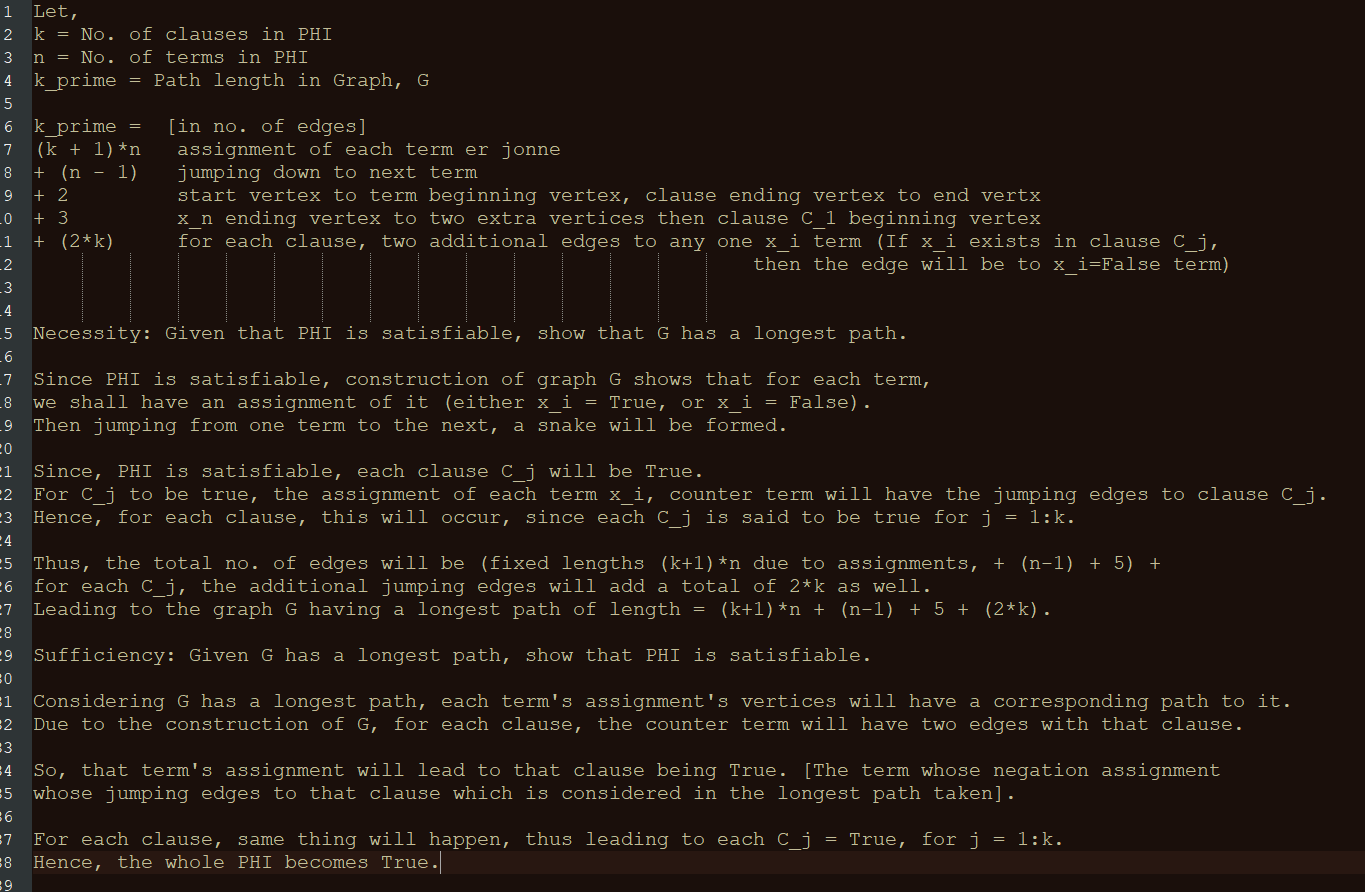
\includegraphics[scale=0.20]{longest-path-algo-proof.png}
%     \caption{Messenger theke newa}
%     \label{fig:my_label}
% \end{figure}

%%% References add korish k kare bolosh? %%%%
\begin{section}{Variations}
    \begin{frame}{Polynomial time variations}
    \centering
    \scalebox{1}{%
    \begin{tabular}{|c|c|c|} \hline
    \textbf{Special graphs} & \textbf{Complexity} & \textbf{Comments} \\ \hline \hline
    Tree & Linear & Dijkstra's algorithm \cite{BULTERMAN200293}\\ \hline 
    Cacti Graph & $O(n^{2})$ & \cite{10.1007/978-3-540-30551-4_74} \\ \hline
    Bipartite Permutation Graph & Linear &  \cite{UEHARA200771}  \\ \hline
    Directed Acyclic Graph & Linear & Dynamic approach \\ \hline
    Interval Graph & $O(n^{4})$ & Dynamic approach \cite{inproceedings} \\ \hline
    Circular Arc Graph & $O(n^{4})$ & Dynamic approach \cite{MERTZIOS2014383} \\ \hline
    Co-compatibility Graph & $O(n^{7})$ & From Hasse diagram \cite{Ioannidou2013} \\ \hline 
\end{tabular}}
%% https://stackoverflow.com/questions/2978125/beamer-make-itemize-and-space-occupied-disappear
    \begin{itemize}
        \item <only@1> Tree is undirected acyclic graph.Dijkstra proposed an algorithm for this in 1960.
        \item <only@2>Cacti is a special kind of block graph which each block is a cycle.Two cycle share at most one vertex which is a separator.
        \item <only@3>The class of bipartite permutation graphs is the intersection of two well known graph classes: bipartite graphs and permutation graphs. A complete bipartite decomposition of a bipartite permutation graph is proposed in this reference.
        \item <only@4>The longest path for general graphs does not have a optimal substructure property but it has for weighted directed acyclic graphs.
        \item <only@5>An interval graph is an undirected graph formed from a set of intervals on the real line, with a vertex for each interval and an edge between vertices whose intervals intersect. It is the intersection graph of the intervals.
        \item <only@6>In graph theory, a circular-arc graph is the intersection graph of a set of arcs on the circle.It has one vertex for each arc in the set, and an edge between every pair of vertices corresponding to arcs that intersect.
        \item <only@7>In graph theory, a comparability graph is an undirected graph that connects pairs of elements that are comparable to each other in a partial order.
    \end{itemize}
\end{frame}




\begin{frame}{Observation}
    \begin{itemize}
        \item The longest path problem is solvable in polynomial time 
on any class of graphs with bounded tree-width or bounded clique-width, 
such as the distance-hereditary graphs.
        \item Finally, it is clearly NP-hard 
on all graph classes on which the Hamiltonian path problem is NP-hard, 
such as on split graphs, circle graphs, and planar graphs.
    \end{itemize}
    
\end{frame}

% \begin{frame}{Polynomial time variations}
%     \centering
%     \scalebox{0.75}{%
%     \begin{tabular}{|c|c|c|} \hline
%     \textbf{Special graphs} & \textbf{Complexity} & \textbf{Comments} \\ \hline \hline
%     Tree & Linear & Dijkstra's algorithm  \citep{BULTERMAN200293}\\ \hline 
%     Bipertite Permutation Graph & Linear &  \citep{UEHARA200771}  \\ \hline
%     Cactus Graph & Linear & \citep{10.1007/978-3-540-30551-4_74} \\ \hline
%     Directed Acyclic Graph & Linear & Dynamic approach \\ \hline
%     Interval Graph & $O(n^{4})$ & Dynamic approach \citep{inproceedings} \\ \hline
%     Circular Arc Graph & Polynomial & Dynamic approach \citep{MERTZIOS2014383} \\ \hline
%     Co-compatibility Graph & $O(n^{7})$ & Based on Hasse diagram \\ \hline 
    
%     \end{tabular}}
% \end{frame}
% \begin{frame}{Observation}
%     \begin{itemize}
%         \item The longest path problem is solvable in polynomial time 
% on any class of graphs with bounded tree-width or bounded clique-width, 
% such as the distance-hereditary graphs.
%         \item Finally, it is clearly NP-hard 
% on all graph classes on which the Hamiltonian path problem is NP-hard, 
% such as on split graphs, circle graphs, and planar graphs.
%     \end{itemize}
    
% \end{frame}


\end{section}
\begin{section}{Problems that Longest Path Problem Reduces To}
    \subfile{files_1505010/reduces_to.tex}
\end{section}

\end{section}


\begin{frame}[allowframebreaks]{References}
    \bibliographystyle{unsrt}
    % \bibliographystyle{plainnat}
    \bibliography{bibliography}
    
\end{frame}
  
  

   
%*********************************************************************************************
%**********************************************************************************************
%\begin{frame}\frametitle{}
%  \centering
%    \includemedia[
%  width=0.6\linewidth,height=0.45\linewidth,
%  activate=pageopen,
%  flashvars={
%    modestbranding=1 % no YT logo in control bar
%   &autohide=1       % controlbar autohide
%   &showinfo=0       % no title and other info before start
%  }
%]{}{http://www.youtube.com/v/dISaXUlilkU?rel=0}   % Flash file 
      
%\end{frame}
%%%%%%%%%%%%%%%%%%%%%%%%%%%%%%%%%%%%%%%%%%%%%%%%%%%
\end{document}
